% !TeX program = lualatex
% ALIUS Bulletin native visual reconstruction source.
% Generated from off-repo reference layout data; does not include or input a pre-existing article PDF.
\ifdefined\ALIUSIssueBuild
\else
\documentclass{article}
\usepackage[paperwidth=595.2756bp,paperheight=841.8898bp,margin=0bp]{geometry}
\usepackage{graphicx}
\usepackage{xcolor}
\usepackage{tikz}
\usepackage{iftex}
\usepackage[hidelinks]{hyperref}
\ifPDFTeX
  \usepackage[T1]{fontenc}
  \usepackage[utf8]{inputenc}
  \usepackage{textcomp}
  \usepackage{amssymb}
\else
  \usepackage{fontspec}
\fi
\pagestyle{empty}
\fi
\ifPDFTeX
  \providecommand{\ALIUSDeclareUnicodeFallbacks}{%
    \DeclareUnicodeCharacter{00AC}{\ensuremath{\neg}}%
    \DeclareUnicodeCharacter{00BE}{\ensuremath{\frac{3}{4}}}%
    \DeclareUnicodeCharacter{0101}{\=a}%
    \DeclareUnicodeCharacter{0107}{\'c}%
    \DeclareUnicodeCharacter{012B}{\=\i}%
    \DeclareUnicodeCharacter{0131}{\i}%
    \DeclareUnicodeCharacter{0142}{\l}%
    \DeclareUnicodeCharacter{015B}{\'s}%
    \DeclareUnicodeCharacter{016B}{\=u}%
    \DeclareUnicodeCharacter{025C}{q}%
    \DeclareUnicodeCharacter{0278}{t}%
    \DeclareUnicodeCharacter{02AE}{Th}%
    \DeclareUnicodeCharacter{02B0}{ff}%
    \DeclareUnicodeCharacter{02B4}{ffi}%
    \DeclareUnicodeCharacter{02BE}{ft}%
    \DeclareUnicodeCharacter{02BF}{fi}%
    \DeclareUnicodeCharacter{02C0}{fl}%
    \DeclareUnicodeCharacter{02C1}{fi}%
    \DeclareUnicodeCharacter{02D9}{Th}%
    \DeclareUnicodeCharacter{02EF}{gy}%
    \DeclareUnicodeCharacter{0394}{\ensuremath{\Delta}}%
    \DeclareUnicodeCharacter{03B2}{\ensuremath{\beta}}%
    \DeclareUnicodeCharacter{03BA}{\ensuremath{\kappa}}%
    \DeclareUnicodeCharacter{068D}{-}%
    \DeclareUnicodeCharacter{08BC}{ti}%
    \DeclareUnicodeCharacter{099E}{ti}%
    \DeclareUnicodeCharacter{1E43}{\d{m}}%
    \DeclareUnicodeCharacter{1E47}{\d{n}}%
    \DeclareUnicodeCharacter{1E63}{\d{s}}%
    \DeclareUnicodeCharacter{201C}{``}%
    \DeclareUnicodeCharacter{201D}{''}%
    \DeclareUnicodeCharacter{2260}{\ensuremath{\neq}}%
    \DeclareUnicodeCharacter{25A1}{\ensuremath{\square}}%
  }%
  \ifdefined\ALIUSIssueBuild\else\ALIUSDeclareUnicodeFallbacks\fi
  \providecommand{\ALIUSFontLatoLight}{\fontfamily{lato-LF}\fontseries{l}\selectfont}
  \providecommand{\ALIUSFontLatoRegular}{\fontfamily{lato-LF}\fontseries{m}\selectfont}
  \providecommand{\ALIUSFontLatoItalic}{\fontfamily{lato-LF}\fontseries{m}\itshape}
  \providecommand{\ALIUSFontLatoLightItalic}{\fontfamily{lato-LF}\fontseries{l}\itshape}
  \providecommand{\ALIUSFontCormorantRegular}{\fontfamily{CormorantGaramond-LF}\fontseries{m}\selectfont}
  \providecommand{\ALIUSFontCormorantLight}{\fontfamily{CormorantGaramond-LF}\fontseries{l}\selectfont}
  \providecommand{\ALIUSFontCormorantMedium}{\fontfamily{CormorantGaramond-LF}\fontseries{medium}\selectfont}
  \providecommand{\ALIUSFontCormorantBold}{\fontfamily{CormorantGaramond-LF}\fontseries{b}\selectfont}
  \providecommand{\ALIUSFontCormorantItalic}{\fontfamily{CormorantGaramond-LF}\fontseries{m}\itshape}
  \providecommand{\ALIUSFontTimes}{\fontfamily{ptm}\selectfont}
  \providecommand{\ALIUSFontCalibri}{\fontfamily{phv}\selectfont}
  \providecommand{\ALIUSFontCambria}{\fontfamily{ptm}\selectfont}
  \providecommand{\ALIUSFontSymbolFallback}{\fontfamily{ptm}\selectfont}
\else
  \providecommand{\ALIUSFontLatoLight}{\fontspec{Lato Light}}
  \providecommand{\ALIUSFontLatoRegular}{\fontspec{Lato Regular}}
  \providecommand{\ALIUSFontLatoItalic}{\fontspec{Lato Italic}}
  \providecommand{\ALIUSFontLatoLightItalic}{\fontspec{Lato Light Italic}}
  \providecommand{\ALIUSFontCormorantRegular}{\fontspec{Cormorant Garamond Regular}}
  \providecommand{\ALIUSFontCormorantLight}{\fontspec{Cormorant Garamond Light}}
  \providecommand{\ALIUSFontCormorantMedium}{\fontspec{Cormorant Garamond Medium}}
  \providecommand{\ALIUSFontCormorantBold}{\fontspec{Cormorant Garamond Bold}}
  \providecommand{\ALIUSFontCormorantItalic}{\fontspec{Cormorant Garamond Italic}}
  \providecommand{\ALIUSFontTimes}{\fontspec{Times New Roman}}
  \providecommand{\ALIUSFontCalibri}{\fontspec{Calibri}}
  \providecommand{\ALIUSFontCambria}{\fontspec{Cambria}}
  \providecommand{\ALIUSFontSymbolFallback}{\fontspec{Times New Roman}}
\fi
\providecommand{\ALIUSPullQuoteOpen}{\textquotedblleft}
\providecommand{\ALIUSPullQuoteClose}{\textquotedblright}
\definecolor{ALIUSC000000}{HTML}{000000}
\definecolor{ALIUSC1A1718}{HTML}{1A1718}
\definecolor{ALIUSC1F8135}{HTML}{1F8135}
\definecolor{ALIUSC595959}{HTML}{595959}
\definecolor{ALIUSC767171}{HTML}{767171}
\definecolor{ALIUSC7F7F7F}{HTML}{7F7F7F}
\definecolor{ALIUSCFFFFFF}{HTML}{FFFFFF}
\providecommand{\ALIUSPlacedText}[6]{%
  \node[anchor=north west,inner sep=0pt,outer sep=0pt,text=#4] at (#1bp,-#2bp) {%
    \resizebox{#3bp}{!}{{#5\fontsize{#6bp}{#6bp}\selectfont #6\kern0pt}}%
  };%
}
\providecommand{\ALIUSPlacedTextContent}[7]{%
  \node[anchor=north west,inner sep=0pt,outer sep=0pt,text=#4] at (#1bp,-#2bp) {%
    \resizebox{#3bp}{!}{{#5\fontsize{#6bp}{#6bp}\selectfont #7}}%
  };%
}
\ifdefined\ALIUSIssueBuild
\else
\begin{document}
\fi
% Page 1
\thispagestyle{empty}
\noindent
\begin{tikzpicture}[remember picture,overlay,x=1bp,y=1bp,shift={(current page.north west)}]
  \fill[ALIUSC767171] (76.253bp,-777.566bp) rectangle ++(443.378bp,-0.233bp);
  \fill[ALIUSC1F8135] (379.224bp,-143.168bp) rectangle ++(93.993bp,-0.233bp);
  \fill[ALIUSC1F8135] (379.224bp,-202.177bp) rectangle ++(85.830bp,-0.233bp);
  \fill[ALIUSC1F8135] (379.224bp,-271.447bp) rectangle ++(67.638bp,-0.233bp);
  \ALIUSPlacedTextContent{83.143}{81.134}{153.983}{ALIUSC000000}{\ALIUSFontLatoRegular}{18.426}{Dennett Explained}
  \ALIUSPlacedTextContent{83.016}{119.582}{118.993}{ALIUSC000000}{\ALIUSFontLatoLight}{15.627}{An interview with}
  \ALIUSPlacedTextContent{379.224}{119.763}{80.429}{ALIUSC000000}{\ALIUSFontLatoRegular}{11.662}{Daniel Dennett}
  \ALIUSPlacedTextContent{379.224}{133.721}{95.669}{ALIUSC1F8135}{\ALIUSFontLatoLight}{8.863}{daniel.dennett@tufts.edu}
  \ALIUSPlacedTextContent{83.016}{138.277}{124.377}{ALIUSC000000}{\ALIUSFontLatoLight}{18.426}{Daniel Dennett}
  \ALIUSPlacedTextContent{379.224}{144.217}{99.522}{ALIUSC000000}{\ALIUSFontLatoLight}{8.863}{Department of Philosophy}
  \ALIUSPlacedTextContent{379.224}{154.712}{98.616}{ALIUSC000000}{\ALIUSFontLatoLight}{8.863}{Tufts University, MA, USA}
  \ALIUSPlacedTextContent{83.016}{170.154}{149.311}{ALIUSC000000}{\ALIUSFontLatoLight}{12.595}{by Brendan Fleig-Goldstein}
  \ALIUSPlacedTextContent{379.224}{178.772}{126.479}{ALIUSC000000}{\ALIUSFontLatoRegular}{11.662}{Brendan Fleig-Goldstein}
  \ALIUSPlacedTextContent{83.016}{185.314}{126.925}{ALIUSC000000}{\ALIUSFontLatoLight}{12.595}{and Daniel A. Friedman}
  \ALIUSPlacedTextContent{379.224}{192.729}{87.597}{ALIUSC1F8135}{\ALIUSFontLatoLight}{8.863}{fleiggoldstein@pitt.edu}
  \ALIUSPlacedTextContent{379.224}{203.225}{102.035}{ALIUSC000000}{\ALIUSFontLatoLight}{8.863}{Department of History and}
  \ALIUSPlacedTextContent{379.224}{213.720}{83.569}{ALIUSC000000}{\ALIUSFontLatoLight}{8.863}{Philosophy of Science}
  \ALIUSPlacedTextContent{379.224}{224.216}{124.942}{ALIUSC000000}{\ALIUSFontLatoLight}{8.863}{University of Pittsburgh, PA, USA}
  \ALIUSPlacedTextContent{379.224}{248.042}{99.297}{ALIUSC000000}{\ALIUSFontLatoRegular}{11.662}{Daniel A. Friedman}
  % ALIUS normalized citation panel begin
  % ALIUS normalized citation panel text: Cite as: Dennett, D., Fleig-Goldstein, B. \& Friedman, D. (2019). Dennett Explained. An interview with Daniel Dennett. ALIUS Bulletin
  \fill[white] (81.516bp,-256.747bp) rectangle ++(276.793bp,-63.937bp);
  \node[anchor=north west,inner sep=0pt,outer sep=0pt,text=ALIUSC000000] at (83.016bp,-258.747bp) {\begin{minipage}{273.793bp}{\ALIUSFontLatoLight\fontsize{9.200bp}{10.700bp}\selectfont\raggedright Cite as: Dennett, D., Fleig-Goldstein, B. \& Friedman, D. (2019). Dennett Explained. An interview with Daniel Dennett. ALIUS Bulletin\par}\end{minipage}};
  \node[anchor=north west,inner sep=0pt,outer sep=0pt,text=ALIUSC1F8135] at (83.016bp,-295.347bp) {{\ALIUSFontLatoLight\fontsize{8.600bp}{8.600bp}\selectfont\href{https://doi.org/10.34700/7gkw-zh08}{https://doi.org/10.34700/7gkw-zh08}}};
  % ALIUS normalized citation panel end
  \ALIUSPlacedTextContent{379.224}{262.000}{69.401}{ALIUSC1F8135}{\ALIUSFontLatoLight}{8.863}{dfri@stanford.edu}
  \ALIUSPlacedTextContent{366.809}{270.408}{3.810}{ALIUSC000000}{\ALIUSFontLatoLight}{9.796}{,}
  \ALIUSPlacedTextContent{379.224}{272.495}{88.135}{ALIUSC000000}{\ALIUSFontLatoLight}{8.863}{Department of Biology}
  \ALIUSPlacedTextContent{379.224}{282.991}{108.112}{ALIUSC000000}{\ALIUSFontLatoLight}{8.863}{Stanford University, CA, USA}
  \ALIUSPlacedTextContent{77.652}{327.184}{48.871}{ALIUSC000000}{\ALIUSFontLatoLight}{12.471}{Abstract}
  \ALIUSPlacedTextContent{77.652}{346.234}{442.784}{ALIUSC000000}{\ALIUSFontLatoLight}{11.662}{Throughout his long career, Professor Daniel Dennett has been notable for bringing}
  \ALIUSPlacedTextContent{77.652}{360.228}{442.773}{ALIUSC000000}{\ALIUSFontLatoLight}{11.662}{together the ideas of academic philosophy, workbench scientists, artificial intelligence}
  \ALIUSPlacedTextContent{77.652}{374.222}{442.782}{ALIUSC000000}{\ALIUSFontLatoLight}{11.662}{pioneers, and even "cultish" intellectual figures like Julian Jaynes and J.J. Gibson. In this}
  \ALIUSPlacedTextContent{77.652}{388.216}{442.784}{ALIUSC000000}{\ALIUSFontLatoLight}{11.662}{interview, Dennett discusses his philosophical roots, as well as his thoughts on Freud,}
  \ALIUSPlacedTextContent{77.652}{402.210}{442.775}{ALIUSC000000}{\ALIUSFontLatoLight}{11.662}{predictive processing, psychedelics, consciousness, and ancient Athens. Dennett believes}
  \ALIUSPlacedTextContent{77.652}{416.204}{442.778}{ALIUSC000000}{\ALIUSFontLatoLight}{11.662}{that philosophers have the ability to criticize and contribute to the science of the mind, and}
  \ALIUSPlacedTextContent{77.652}{430.198}{442.772}{ALIUSC000000}{\ALIUSFontLatoLight}{11.662}{speaks to the virtues of cross-disciplinary glances and "hybrid vigor." He believes that}
  \ALIUSPlacedTextContent{77.652}{444.192}{442.776}{ALIUSC000000}{\ALIUSFontLatoLight}{11.662}{psychoactive drugs have potential scientific and therapeutic value. Experimenting with}
  \ALIUSPlacedTextContent{77.652}{458.186}{442.780}{ALIUSC000000}{\ALIUSFontLatoLight}{11.662}{psychoactive substances, however, should be done within the proper settings, and not left}
  \ALIUSPlacedTextContent{77.652}{472.180}{81.607}{ALIUSC000000}{\ALIUSFontLatoLight}{11.662}{to rogue agents.}
  \ALIUSPlacedTextContent{119.909}{503.655}{382.394}{ALIUSC000000}{\ALIUSFontLatoLightItalic}{10.729}{altered states of consciousness, cognitive science, consciousness, philosophy, psychedelics.}
  \ALIUSPlacedTextContent{77.652}{503.700}{42.252}{ALIUSC000000}{\ALIUSFontLatoLightItalic}{10.623}{keywords:}
  \ALIUSPlacedTextContent{77.652}{533.994}{442.861}{ALIUSC1F8135}{\ALIUSFontLatoLight}{12.128}{Your published works—and interviews—span volumes and fields, conveying complex}
  \ALIUSPlacedTextContent{77.652}{548.687}{362.048}{ALIUSC1F8135}{\ALIUSFontLatoLight}{12.128}{ideas through engaging words and thought experiments. The singular}
  \ALIUSPlacedTextContent{440.467}{548.687}{80.010}{ALIUSC1F8135}{\ALIUSFontLatoLightItalic}{12.128}{Intuition Pumps}
  \ALIUSPlacedTextContent{77.652}{563.148}{150.115}{ALIUSC1F8135}{\ALIUSFontLatoLightItalic}{12.128}{and Other Tools for Thinking}
  \ALIUSPlacedTextContent{230.331}{563.148}{290.152}{ALIUSC1F8135}{\ALIUSFontLatoLight}{12.128}{(2013b) breaks the fourth wall of being a philosophy}
  \ALIUSPlacedTextContent{77.652}{577.842}{420.646}{ALIUSC1F8135}{\ALIUSFontLatoLight}{12.128}{professor, allowing the reader access to your mental processes. Works such as}
  \ALIUSPlacedTextContent{499.940}{577.842}{20.572}{ALIUSC1F8135}{\ALIUSFontLatoLightItalic}{12.128}{The}
  \ALIUSPlacedTextContent{77.652}{592.302}{38.890}{ALIUSC1F8135}{\ALIUSFontLatoLightItalic}{12.128}{Mind's I}
  \ALIUSPlacedTextContent{116.555}{592.302}{403.845}{ALIUSC1F8135}{\ALIUSFontLatoLight}{12.128}{(Hofstadter \& Dennett, 1982) transcend genres as well as single authorship,}
  \ALIUSPlacedTextContent{77.652}{606.996}{442.839}{ALIUSC1F8135}{\ALIUSFontLatoLight}{12.128}{positing deep questions to the philosophical, while also offering a doorway into}
  \ALIUSPlacedTextContent{77.652}{621.456}{173.393}{ALIUSC1F8135}{\ALIUSFontLatoLight}{12.128}{philosophy for the inexperienced.}
  \ALIUSPlacedTextContent{251.083}{621.456}{120.835}{ALIUSC1F8135}{\ALIUSFontLatoLightItalic}{12.128}{Darwin's Dangerous Idea}
  \ALIUSPlacedTextContent{371.942}{621.456}{148.564}{ALIUSC1F8135}{\ALIUSFontLatoLight}{12.128}{(Dennett, 1996) is as a clear}
  \ALIUSPlacedTextContent{77.652}{636.150}{443.125}{ALIUSC1F8135}{\ALIUSFontLatoLight}{12.128}{a defense of evolution now, as it was before the current genomics era in biology. Even}
  \ALIUSPlacedTextContent{77.652}{650.611}{442.798}{ALIUSC1F8135}{\ALIUSFontLatoLight}{12.128}{in your articles published in philosophy journals, your work retains an accessible feel to}
  \ALIUSPlacedTextContent{77.652}{665.305}{442.818}{ALIUSC1F8135}{\ALIUSFontLatoLight}{12.128}{it. Such engaging and radically interactive types of philosophy are rare overall. The}
  \ALIUSPlacedTextContent{77.652}{679.765}{440.521}{ALIUSC1F8135}{\ALIUSFontLatoLight}{12.128}{effect of your philosophical style has been to buck the typical insularity and over-}
  \ALIUSPlacedTextContent{77.652}{694.459}{442.881}{ALIUSC1F8135}{\ALIUSFontLatoLight}{12.128}{professionalized nature of academic philosophy, providing an inroad for many people}
  \ALIUSPlacedTextContent{77.652}{708.919}{442.841}{ALIUSC1F8135}{\ALIUSFontLatoLight}{12.128}{into some of the most valuable aspects of philosophical thinking, and also spurring an}
  \ALIUSPlacedTextContent{77.652}{723.613}{378.954}{ALIUSC1F8135}{\ALIUSFontLatoLight}{12.128}{incredible amount of students into various areas of the cognitive sciences.}
  \ALIUSPlacedTextContent{77.652}{783.303}{117.883}{ALIUSC767171}{\ALIUSFontLatoLight}{10.729}{ALIUS Bulletin n°3 (2019)}
  \ALIUSPlacedTextContent{402.025}{783.303}{116.144}{ALIUSC767171}{\ALIUSFontLatoLight}{10.729}{aliusresearch.org/bulletin}
\end{tikzpicture}
\null
\newpage
% Page 2
\thispagestyle{empty}
\noindent\begin{tikzpicture}[remember picture,overlay,x=1bp,y=1bp,shift={(current page.north west)}]
  \fill[ALIUSC767171] (76.253bp,-65.268bp) rectangle ++(443.378bp,-0.233bp);
  \fill[ALIUSC767171] (76.253bp,-777.332bp) rectangle ++(443.378bp,-0.466bp);
  \ALIUSPlacedTextContent{77.652}{46.516}{164.318}{ALIUSC767171}{\ALIUSFontLatoLight}{10.729}{Daniel Dennett - Dennett Explained}
  \ALIUSPlacedTextContent{505.773}{46.516}{14.471}{ALIUSC767171}{\ALIUSFontLatoLight}{10.729}{12}
  \ALIUSPlacedTextContent{77.652}{81.286}{442.878}{ALIUSC1F8135}{\ALIUSFontLatoLight}{12.128}{Where do you believe this strategy came from, and how has your perspective on}
  \ALIUSPlacedTextContent{77.652}{95.980}{274.796}{ALIUSC1F8135}{\ALIUSFontLatoLight}{12.128}{communicating philosophy evolved over your career?}
  \ALIUSPlacedTextContent{77.652}{122.039}{443.760}{ALIUSC000000}{\ALIUSFontCormorantMedium}{13.528}{Well, my two chief advisors were W.V.O. Quine and Gilbert Ryle, who were both}
  \ALIUSPlacedTextContent{77.652}{138.366}{443.733}{ALIUSC000000}{\ALIUSFontCormorantMedium}{13.528}{fine writers (who tried never to write a boring sentence and pretty well succeeded,}
  \ALIUSPlacedTextContent{77.652}{154.925}{443.676}{ALIUSC000000}{\ALIUSFontCormorantMedium}{13.528}{at least for philosophically adept readers). I've also had, since I was an}
  \ALIUSPlacedTextContent{77.652}{171.485}{443.721}{ALIUSC000000}{\ALIUSFontCormorantMedium}{13.528}{undergraduate, a suspicion of philosophers who seemed to go out of their way to}
  \ALIUSPlacedTextContent{77.652}{187.811}{443.644}{ALIUSC000000}{\ALIUSFontCormorantMedium}{13.528}{make their work forbidding and technical and "deep." They didn't seem to want to}
  \ALIUSPlacedTextContent{77.652}{204.371}{160.223}{ALIUSC000000}{\ALIUSFontCormorantMedium}{13.528}{explain what they were up to!}
  \ALIUSPlacedTextContent{77.652}{232.655}{442.870}{ALIUSC1F8135}{\ALIUSFontLatoLight}{12.128}{If you were to "start it all over" as a young person with the same mindset in 2018, do}
  \ALIUSPlacedTextContent{77.652}{247.115}{442.896}{ALIUSC1F8135}{\ALIUSFontLatoLight}{12.128}{you think you would have stayed in academia and tried to break out again, or might you}
  \ALIUSPlacedTextContent{77.652}{261.809}{312.350}{ALIUSC1F8135}{\ALIUSFontLatoLight}{12.128}{have explored other avenues for communicating philosophy?}
  \ALIUSPlacedTextContent{77.652}{287.869}{443.679}{ALIUSC000000}{\ALIUSFontCormorantMedium}{13.528}{The problem is that the audience for philosophy today includes many who don't}
  \ALIUSPlacedTextContent{77.652}{304.428}{443.559}{ALIUSC000000}{\ALIUSFontCormorantMedium}{13.528}{have the time or patience or, in the end, interest to really dig into a topic; they want}
  \ALIUSPlacedTextContent{77.652}{320.755}{443.694}{ALIUSC000000}{\ALIUSFontCormorantMedium}{13.528}{instant gratification. I once wrote a little fable about this, in my review of Bob}
  \ALIUSPlacedTextContent{77.652}{337.315}{219.989}{ALIUSC000000}{\ALIUSFontCormorantMedium}{13.528}{Nozick's wonderful book (Dennett 1982):}
  \ALIUSPlacedTextContent{132.753}{378.830}{190.467}{ALIUSC000000}{\ALIUSFontCormorantMedium}{13.528}{There was once a chap who wanted}
  \ALIUSPlacedTextContent{132.753}{395.390}{182.738}{ALIUSC000000}{\ALIUSFontCormorantMedium}{13.528}{to know the meaning of life, so he}
  \ALIUSPlacedTextContent{132.753}{411.950}{201.732}{ALIUSC000000}{\ALIUSFontCormorantMedium}{13.528}{walked a thousand miles and climbed}
  \ALIUSPlacedTextContent{132.753}{428.276}{215.704}{ALIUSC000000}{\ALIUSFontCormorantMedium}{13.528}{to the high mountaintop where the wise}
  \ALIUSPlacedTextContent{132.753}{444.836}{220.901}{ALIUSC000000}{\ALIUSFontCormorantMedium}{13.528}{guru lived. "Will you tell me the meaning}
  \ALIUSPlacedTextContent{132.753}{461.162}{93.666}{ALIUSC000000}{\ALIUSFontCormorantMedium}{13.528}{of life?" he asked.}
  \ALIUSPlacedTextContent{132.753}{477.722}{193.037}{ALIUSC000000}{\ALIUSFontCormorantMedium}{13.528}{"Certainly," replied the guru, "but if}
  \ALIUSPlacedTextContent{132.753}{494.281}{192.630}{ALIUSC000000}{\ALIUSFontCormorantMedium}{13.528}{you want to understand my answer,}
  \ALIUSPlacedTextContent{132.753}{510.608}{215.663}{ALIUSC000000}{\ALIUSFontCormorantMedium}{13.528}{you must first master recursive function}
  \ALIUSPlacedTextContent{132.753}{527.167}{171.638}{ALIUSC000000}{\ALIUSFontCormorantMedium}{13.528}{theory and mathematical logic."}
  \ALIUSPlacedTextContent{132.753}{543.727}{90.197}{ALIUSC000000}{\ALIUSFontCormorantMedium}{13.528}{"You're kidding"}
  \ALIUSPlacedTextContent{132.753}{560.053}{66.211}{ALIUSC000000}{\ALIUSFontCormorantMedium}{13.528}{"No, really."}
  \ALIUSPlacedTextContent{132.753}{576.613}{111.298}{ALIUSC000000}{\ALIUSFontCormorantMedium}{13.528}{"Well, then...skip it."}
  \ALIUSPlacedTextContent{132.753}{593.173}{81.272}{ALIUSC000000}{\ALIUSFontCormorantMedium}{13.528}{"Suit yourself."}
  \ALIUSPlacedTextContent{77.652}{636.383}{442.884}{ALIUSC1F8135}{\ALIUSFontLatoLight}{12.128}{You playfully characterized your earliest venture into academic philosophy as a mission}
  \ALIUSPlacedTextContent{77.652}{651.077}{442.878}{ALIUSC1F8135}{\ALIUSFontLatoLight}{12.128}{to "Refute Quine," an endeavor which ultimately led you to become something of the}
  \ALIUSPlacedTextContent{77.652}{665.538}{442.877}{ALIUSC1F8135}{\ALIUSFontLatoLight}{12.128}{"village Quinian" by the time you had arrived at Oxford for graduate school. Following}
  \ALIUSPlacedTextContent{77.652}{680.232}{442.861}{ALIUSC1F8135}{\ALIUSFontLatoLight}{12.128}{Quine, you view science and philosophy as continuous (Ross, Brook, \& Thompson,}
  \ALIUSPlacedTextContent{77.652}{694.692}{442.796}{ALIUSC1F8135}{\ALIUSFontLatoLight}{12.128}{2000). This led you to reject the analytic-synthetic distinction, accept the}
  \ALIUSPlacedTextContent{77.652}{709.386}{442.826}{ALIUSC1F8135}{\ALIUSFontLatoLight}{12.128}{indeterminacy of translation thesis, and find affinity with American pragmatic traditions}
  \ALIUSPlacedTextContent{77.652}{723.846}{442.863}{ALIUSC1F8135}{\ALIUSFontLatoLight}{12.128}{(Hookway, 2016). You stated that Quine's view of a philosopher's primary role is to}
  \ALIUSPlacedTextContent{77.652}{738.540}{442.836}{ALIUSC1F8135}{\ALIUSFontLatoLight}{12.128}{"[provide] the conceptual clarifications and underpinnings for theories that are}
  \ALIUSPlacedTextContent{77.652}{783.303}{117.883}{ALIUSC767171}{\ALIUSFontLatoLight}{10.729}{ALIUS Bulletin n°3 (2019)}
  \ALIUSPlacedTextContent{402.025}{783.303}{116.144}{ALIUSC767171}{\ALIUSFontLatoLight}{10.729}{aliusresearch.org/bulletin}
\end{tikzpicture}
\null
\newpage
% Page 3
\thispagestyle{empty}
\noindent\begin{tikzpicture}[remember picture,overlay,x=1bp,y=1bp,shift={(current page.north west)}]
  \fill[ALIUSC767171] (76.253bp,-65.268bp) rectangle ++(443.378bp,-0.233bp);
  \fill[ALIUSC767171] (76.253bp,-777.332bp) rectangle ++(443.378bp,-0.466bp);
  \ALIUSPlacedTextContent{77.652}{46.516}{164.318}{ALIUSC767171}{\ALIUSFontLatoLight}{10.729}{Daniel Dennett - Dennett Explained}
  \ALIUSPlacedTextContent{505.773}{46.516}{14.471}{ALIUSC767171}{\ALIUSFontLatoLight}{10.729}{13}
  \ALIUSPlacedTextContent{77.652}{81.286}{442.874}{ALIUSC1F8135}{\ALIUSFontLatoLight}{12.128}{testable, empirical, scientific," though noted that "he didn't get much chance to actually}
  \ALIUSPlacedTextContent{77.652}{95.746}{442.861}{ALIUSC1F8135}{\ALIUSFontLatoLight}{12.128}{do philosophy in this vein" (Dennett, 2003). This in some ways contextualizes your place}
  \ALIUSPlacedTextContent{77.652}{110.440}{442.790}{ALIUSC1F8135}{\ALIUSFontLatoLight}{12.128}{in the conceptual landscape of philosophy: At a deep level, the perspective of Quine}
  \ALIUSPlacedTextContent{77.652}{124.901}{442.892}{ALIUSC1F8135}{\ALIUSFontLatoLight}{12.128}{deeply resonates through your thinking. Yet methodologically, you have diverged from}
  \ALIUSPlacedTextContent{77.652}{139.594}{442.866}{ALIUSC1F8135}{\ALIUSFontLatoLight}{12.128}{Quine and his ilk in that you rarely resort to the technical, mathematical, or otherwise}
  \ALIUSPlacedTextContent{77.652}{154.288}{420.048}{ALIUSC1F8135}{\ALIUSFontLatoLight}{12.128}{formal presentations of your ideas that characterizes much of analytic philosophy.}
  \ALIUSPlacedTextContent{77.652}{180.410}{233.640}{ALIUSC1F8135}{\ALIUSFontLatoLight}{12.128}{First, do you find these points to be accurate?}
  \ALIUSPlacedTextContent{84.777}{206.703}{13.549}{ALIUSC000000}{\ALIUSFontCormorantMedium}{13.528}{es!}
  \ALIUSPlacedTextContent{77.652}{208.427}{7.125}{ALIUSC000000}{\ALIUSFontCormorantMedium}{11.662}{Y}
  \ALIUSPlacedTextContent{77.652}{234.754}{443.017}{ALIUSC1F8135}{\ALIUSFontLatoLight}{12.128}{Second, today, what do you see as the biggest disagreement that you have with Quine}
  \ALIUSPlacedTextContent{77.652}{249.448}{251.892}{ALIUSC1F8135}{\ALIUSFontLatoLight}{12.128}{methodologically, and also concerning cognition?}
  \ALIUSPlacedTextContent{77.652}{275.507}{443.690}{ALIUSC000000}{\ALIUSFontCormorantMedium}{13.528}{Quine, as a logician, wanted to get everything into a strict, well-policed system of}
  \ALIUSPlacedTextContent{77.652}{292.067}{443.585}{ALIUSC000000}{\ALIUSFontCormorantMedium}{13.528}{expression. I viewed that project as hopeless and ill-motivated, but the effort was}
  \ALIUSPlacedTextContent{77.652}{308.627}{295.334}{ALIUSC000000}{\ALIUSFontCormorantMedium}{13.528}{nevertheless full of enlightening challenges and pitfalls.}
  \ALIUSPlacedTextContent{77.652}{336.677}{383.545}{ALIUSC1F8135}{\ALIUSFontLatoLight}{12.128}{In what ways do you feel you changed Quine's mind throughout his career?}
  \ALIUSPlacedTextContent{77.652}{362.737}{443.507}{ALIUSC000000}{\ALIUSFontCormorantMedium}{13.528}{Quine had a long friendship with B.F. Skinner, and simply bought into many of his}
  \ALIUSPlacedTextContent{77.652}{379.297}{443.626}{ALIUSC000000}{\ALIUSFontCormorantMedium}{13.528}{friend's proposed behavioristic simplifications. In those days it really was premature}
  \ALIUSPlacedTextContent{77.652}{395.856}{443.679}{ALIUSC000000}{\ALIUSFontCormorantMedium}{13.528}{to try to hypothesize much in the way of particular neural mechanisms for cognition,}
  \ALIUSPlacedTextContent{77.652}{412.183}{443.794}{ALIUSC000000}{\ALIUSFontCormorantMedium}{13.528}{so behaviorism could be viewed as a prudent noncommittal way of getting an}
  \ALIUSPlacedTextContent{77.652}{428.742}{443.615}{ALIUSC000000}{\ALIUSFontCormorantMedium}{13.528}{account of a system's input-output competence. But I think I got him to see that his}
  \ALIUSPlacedTextContent{77.652}{445.302}{443.744}{ALIUSC000000}{\ALIUSFontCormorantMedium}{13.528}{pure Skinnerian behaviorism was too simple, more of a "nice try" than a "good trick."}
  \ALIUSPlacedTextContent{77.652}{461.628}{443.521}{ALIUSC000000}{\ALIUSFontCormorantMedium}{13.528}{He softened his line on the abandonment of intentional idioms in science after he}
  \ALIUSPlacedTextContent{77.652}{478.188}{446.870}{ALIUSC000000}{\ALIUSFontCormorantMedium}{13.528}{saw that there was a rather Quinian way of handling them—my "intentional stance."}
  \ALIUSPlacedTextContent{77.652}{506.239}{442.947}{ALIUSC1F8135}{\ALIUSFontLatoLight}{12.128}{Your early career was characterized by the fact that you took the time to learn}
  \ALIUSPlacedTextContent{77.652}{520.932}{442.895}{ALIUSC1F8135}{\ALIUSFontLatoLight}{12.128}{neuroscience and psychology and incorporated these studies into philosophy of mind}
  \ALIUSPlacedTextContent{77.652}{535.393}{443.078}{ALIUSC1F8135}{\ALIUSFontLatoLight}{12.128}{and philosophy of language. For many years you have argued against philosophers and}
  \ALIUSPlacedTextContent{77.652}{550.087}{442.836}{ALIUSC1F8135}{\ALIUSFontLatoLight}{12.128}{scientists alike on what the implications of scientific findings are for the study of}
  \ALIUSPlacedTextContent{77.652}{564.547}{442.735}{ALIUSC1F8135}{\ALIUSFontLatoLight}{12.128}{consciousness (e.g., neuroscientific studies purporting to show that we do not have free}
  \ALIUSPlacedTextContent{77.652}{579.241}{442.924}{ALIUSC1F8135}{\ALIUSFontLatoLight}{12.128}{will). This sort of pioneering interdisciplinary work sowed the seeds for the approach}
  \ALIUSPlacedTextContent{77.652}{593.702}{442.868}{ALIUSC1F8135}{\ALIUSFontLatoLight}{12.128}{we take here at ALIUS: to generate scientific knowledge about "consciousness" using}
  \ALIUSPlacedTextContent{77.652}{608.395}{442.870}{ALIUSC1F8135}{\ALIUSFontLatoLight}{12.128}{diverse methodologies and conceptual frameworks. Further, you have also engaged in}
  \ALIUSPlacedTextContent{77.652}{622.856}{442.898}{ALIUSC1F8135}{\ALIUSFontLatoLight}{12.128}{plausible speculations about as yet unanswered empirical questions, such as how}
  \ALIUSPlacedTextContent{77.652}{637.550}{442.876}{ALIUSC1F8135}{\ALIUSFontLatoLight}{12.128}{hallucinations work, how neurons learn through evolution, and the nature of}
  \ALIUSPlacedTextContent{77.652}{652.010}{442.845}{ALIUSC1F8135}{\ALIUSFontLatoLight}{12.128}{consciousness. In doing so, you have often anticipated future trends in cognitive}
  \ALIUSPlacedTextContent{77.652}{666.704}{442.746}{ALIUSC1F8135}{\ALIUSFontLatoLight}{12.128}{science. For example, in your speculation on hallucinations, you anticipated the essence}
  \ALIUSPlacedTextContent{77.652}{681.164}{442.877}{ALIUSC1F8135}{\ALIUSFontLatoLight}{12.128}{of the predictive processing paradigm (Dennett, 1993). All of these actions comport}
  \ALIUSPlacedTextContent{77.652}{695.858}{443.035}{ALIUSC1F8135}{\ALIUSFontLatoLight}{12.128}{well with the view that science and philosophy are continuous. Nevertheless, there is a}
  \ALIUSPlacedTextContent{77.652}{710.319}{442.878}{ALIUSC1F8135}{\ALIUSFontLatoLight}{12.128}{difference between providing conceptual and clarificatory underpinnings for scientific}
  \ALIUSPlacedTextContent{77.652}{725.012}{442.819}{ALIUSC1F8135}{\ALIUSFontLatoLight}{12.128}{theories, and providing speculative scientific theories themselves—even if it is a matter}
  \ALIUSPlacedTextContent{77.652}{739.706}{53.773}{ALIUSC1F8135}{\ALIUSFontLatoLight}{12.128}{of degree.}
  \ALIUSPlacedTextContent{77.652}{783.303}{117.883}{ALIUSC767171}{\ALIUSFontLatoLight}{10.729}{ALIUS Bulletin n°3 (2019)}
  \ALIUSPlacedTextContent{402.025}{783.303}{116.144}{ALIUSC767171}{\ALIUSFontLatoLight}{10.729}{aliusresearch.org/bulletin}
\end{tikzpicture}
\null
\newpage
% Page 4
\thispagestyle{empty}
\noindent
\begin{tikzpicture}[remember picture,overlay,x=1bp,y=1bp,shift={(current page.north west)}]
  \fill[ALIUSC767171] (76.253bp,-65.268bp) rectangle ++(443.378bp,-0.233bp);
  \fill[ALIUSC767171] (76.253bp,-777.332bp) rectangle ++(443.378bp,-0.466bp);
  \ALIUSPlacedTextContent{77.652}{46.516}{164.318}{ALIUSC767171}{\ALIUSFontLatoLight}{10.729}{Daniel Dennett - Dennett Explained}
  \ALIUSPlacedTextContent{505.773}{46.516}{14.471}{ALIUSC767171}{\ALIUSFontLatoLight}{10.729}{14}
  \ALIUSPlacedTextContent{77.652}{81.286}{442.947}{ALIUSC1F8135}{\ALIUSFontLatoLight}{12.128}{First, when, in your mind, is it appropriate or useful for a philosopher to engage in the}
  \ALIUSPlacedTextContent{77.652}{95.746}{442.837}{ALIUSC1F8135}{\ALIUSFontLatoLight}{12.128}{latter end of this spectrum, i.e., speculating on empirical questions? What is the role of}
  \ALIUSPlacedTextContent{77.652}{110.440}{87.379}{ALIUSC1F8135}{\ALIUSFontLatoLight}{12.128}{this speculation?}
  \ALIUSPlacedTextContent{77.652}{136.500}{443.716}{ALIUSC000000}{\ALIUSFontCormorantMedium}{13.528}{I don't think there are any useful principles or policies here; it is a matter of seeing}
  \ALIUSPlacedTextContent{77.652}{153.059}{443.726}{ALIUSC000000}{\ALIUSFontCormorantMedium}{13.528}{an opportunity and acting on it. I found myself at workshops and other meetings}
  \ALIUSPlacedTextContent{77.652}{169.619}{443.695}{ALIUSC000000}{\ALIUSFontCormorantMedium}{13.528}{where scientists were describing experiments and asking them "what if you gave}
  \ALIUSPlacedTextContent{77.652}{185.945}{443.647}{ALIUSC000000}{\ALIUSFontCormorantMedium}{13.528}{subjects this variation...?" or "how do you know that subjects aren't...?"...and so forth,}
  \ALIUSPlacedTextContent{77.652}{202.505}{443.567}{ALIUSC000000}{\ALIUSFontCormorantMedium}{13.528}{and sometimes the reply would be "that's a great idea, let's try it!" I had enough hits}
  \ALIUSPlacedTextContent{77.652}{219.065}{443.644}{ALIUSC000000}{\ALIUSFontCormorantMedium}{13.528}{with that policy that I got into the habit of thinking about what experiments I would}
  \ALIUSPlacedTextContent{77.652}{235.391}{443.768}{ALIUSC000000}{\ALIUSFontCormorantMedium}{13.528}{run and why. My contributions in such cases are no different from any}
  \ALIUSPlacedTextContent{77.652}{251.951}{443.680}{ALIUSC000000}{\ALIUSFontCormorantMedium}{13.528}{experimenter's suggestions. But perhaps my familiarity with all the "bird's-eye-view"}
  \ALIUSPlacedTextContent{77.652}{268.277}{443.640}{ALIUSC000000}{\ALIUSFontCormorantMedium}{13.528}{issues that philosophers worry about sometimes gives me a better perspective;}
  \ALIUSPlacedTextContent{77.652}{284.837}{443.635}{ALIUSC000000}{\ALIUSFontCormorantMedium}{13.528}{experimenters can get stuck in the trenches and forget where they are on the}
  \ALIUSPlacedTextContent{77.652}{301.396}{60.742}{ALIUSC000000}{\ALIUSFontCormorantMedium}{13.528}{battlefield.}
  \ALIUSPlacedTextContent{77.652}{329.447}{443.069}{ALIUSC1F8135}{\ALIUSFontLatoLight}{12.128}{Second, a perennial question in philosophy of science is whether or not philosophers}
  \ALIUSPlacedTextContent{77.652}{344.141}{442.862}{ALIUSC1F8135}{\ALIUSFontLatoLight}{12.128}{can tell scientists how to do better science. In what ways, if any, do you believe that a}
  \ALIUSPlacedTextContent{77.652}{358.835}{259.745}{ALIUSC1F8135}{\ALIUSFontLatoLight}{12.128}{philosopher can tell a scientist how to do their job?}
  \ALIUSPlacedTextContent{77.652}{384.894}{443.651}{ALIUSC000000}{\ALIUSFontCormorantMedium}{13.528}{Anybody can, in principle, tell scientists how to do better science. Scientists are just}
  \ALIUSPlacedTextContent{77.652}{401.454}{443.702}{ALIUSC000000}{\ALIUSFontCormorantMedium}{13.528}{as vulnerable to illusion, sloppy thinking, unrecognized presuppositions as anyone}
  \ALIUSPlacedTextContent{77.652}{417.780}{443.680}{ALIUSC000000}{\ALIUSFontCormorantMedium}{13.528}{else. And sometimes 'hybrid vigor' is particularly valuable. Schrödinger was no}
  \ALIUSPlacedTextContent{77.652}{434.340}{443.693}{ALIUSC000000}{\ALIUSFontCormorantMedium}{13.528}{biologist, but he certainly gave a major boost to biology in What is Life?. Judea Pearl}
  \ALIUSPlacedTextContent{77.652}{450.666}{443.786}{ALIUSC000000}{\ALIUSFontCormorantMedium}{13.528}{comes to mind as an AI researcher (and a good amateur philosopher!) who has}
  \ALIUSPlacedTextContent{77.652}{467.226}{443.680}{ALIUSC000000}{\ALIUSFontCormorantMedium}{13.528}{developed statistical and mathematical methods that can teach researchers in lots of}
  \ALIUSPlacedTextContent{77.652}{483.786}{440.496}{ALIUSC000000}{\ALIUSFontCormorantMedium}{13.528}{other fields how to do their projects better. I would love to see a curious and well-}
  \ALIUSPlacedTextContent{77.652}{500.112}{443.559}{ALIUSC000000}{\ALIUSFontCormorantMedium}{13.528}{informed poet ask a question that opened the eyes of, say, neuroscientists or (let's be}
  \ALIUSPlacedTextContent{77.652}{516.672}{443.686}{ALIUSC000000}{\ALIUSFontCormorantMedium}{13.528}{ambitious) geologists. But philosophers should be better positioned than most}
  \ALIUSPlacedTextContent{77.652}{533.231}{443.626}{ALIUSC000000}{\ALIUSFontCormorantMedium}{13.528}{others to provide such perspectives because they claim to specialize in thinking the}
  \ALIUSPlacedTextContent{77.652}{549.791}{429.155}{ALIUSC000000}{\ALIUSFontCormorantMedium}{13.528}{unthinkable, expanding the imagination, critiquing the hidden assumptions, etc.}
  \ALIUSPlacedTextContent{134.561}{595.134}{24.676}{ALIUSC7F7F7F}{\ALIUSFontCormorantLight}{46.647}{\ALIUSPullQuoteOpen}
  \ALIUSPlacedTextContent{158.817}{595.134}{247.144}{ALIUSC595959}{\ALIUSFontLatoLight}{14.694}{Anybody can, in principle, tell scientists}
  \ALIUSPlacedTextContent{158.817}{612.627}{247.134}{ALIUSC595959}{\ALIUSFontLatoLight}{14.694}{how to do better science. Scientists are}
  \ALIUSPlacedTextContent{158.817}{630.119}{247.089}{ALIUSC595959}{\ALIUSFontLatoLight}{14.694}{just as vulnerable to illusion, sloppy}
  \ALIUSPlacedTextContent{158.817}{647.612}{247.158}{ALIUSC595959}{\ALIUSFontLatoLight}{14.694}{thinking, unrecognized presuppositions}
  \ALIUSPlacedTextContent{260.741}{663.328}{13.761}{ALIUSC7F7F7F}{\ALIUSFontCormorantLight}{46.647}{\ALIUSPullQuoteClose}
  \ALIUSPlacedTextContent{158.817}{665.105}{94.627}{ALIUSC595959}{\ALIUSFontLatoLight}{14.694}{as anyone else.}
  \ALIUSPlacedTextContent{77.652}{708.919}{442.895}{ALIUSC1F8135}{\ALIUSFontLatoLight}{12.128}{Recently Carhart-Harris and Friston (Carhart-Harris \& Friston, 2010) integrated}
  \ALIUSPlacedTextContent{77.652}{723.613}{442.867}{ALIUSC1F8135}{\ALIUSFontLatoLight}{12.128}{psychiatry with predictive processing and neuroscience to argue that "Freudian}
  \ALIUSPlacedTextContent{77.652}{738.074}{442.871}{ALIUSC1F8135}{\ALIUSFontLatoLight}{12.128}{constructs may have neurobiological substrates." For example they claim that the}
  \ALIUSPlacedTextContent{77.652}{783.303}{117.883}{ALIUSC767171}{\ALIUSFontLatoLight}{10.729}{ALIUS Bulletin n°3 (2019)}
  \ALIUSPlacedTextContent{402.025}{783.303}{116.144}{ALIUSC767171}{\ALIUSFontLatoLight}{10.729}{aliusresearch.org/bulletin}
\end{tikzpicture}
\null
\newpage
% Page 5
\thispagestyle{empty}
\noindent
\begin{tikzpicture}[remember picture,overlay,x=1bp,y=1bp,shift={(current page.north west)}]
  \fill[ALIUSC767171] (76.253bp,-65.268bp) rectangle ++(443.378bp,-0.233bp);
  \fill[ALIUSC767171] (76.253bp,-777.332bp) rectangle ++(443.378bp,-0.466bp);
  \ALIUSPlacedTextContent{77.652}{46.516}{164.318}{ALIUSC767171}{\ALIUSFontLatoLight}{10.729}{Daniel Dennett - Dennett Explained}
  \ALIUSPlacedTextContent{505.773}{46.516}{14.471}{ALIUSC767171}{\ALIUSFontLatoLight}{10.729}{15}
  \ALIUSPlacedTextContent{77.652}{81.286}{442.854}{ALIUSC1F8135}{\ALIUSFontLatoLight}{12.128}{brain's default mode network (DMN) plays a functional role similar to the Freudian ego}
  \ALIUSPlacedTextContent{77.652}{95.746}{442.974}{ALIUSC1F8135}{\ALIUSFontLatoLight}{12.128}{concept, and that distributed cortical activity functionally implements Freud's primary}
  \ALIUSPlacedTextContent{77.652}{110.440}{442.908}{ALIUSC1F8135}{\ALIUSFontLatoLight}{12.128}{and secondary processes (processes that control the id \& ego, respectively). If this}
  \ALIUSPlacedTextContent{77.652}{124.901}{442.867}{ALIUSC1F8135}{\ALIUSFontLatoLight}{12.128}{analysis is correct, then the "virtual governor" you discuss (e.g. in (Dennett, 2018)) may}
  \ALIUSPlacedTextContent{77.652}{139.594}{442.865}{ALIUSC1F8135}{\ALIUSFontLatoLight}{12.128}{not be so virtual, and may instead have a more delineated structural substrate. This}
  \ALIUSPlacedTextContent{77.652}{154.055}{442.876}{ALIUSC1F8135}{\ALIUSFontLatoLight}{12.128}{anatomical network is not a Cartesian Theatre in which a "second transduction" occurs}
  \ALIUSPlacedTextContent{77.652}{168.749}{442.636}{ALIUSC1F8135}{\ALIUSFontLatoLight}{12.128}{(Hobson \& Friston, 2016). Nevertheless, functionally it is like the manager of cerebral}
  \ALIUSPlacedTextContent{77.652}{183.209}{442.852}{ALIUSC1F8135}{\ALIUSFontLatoLight}{12.128}{celebrity (if not the celebrity itself), and in this sense suggests a more centralized}
  \ALIUSPlacedTextContent{77.652}{197.903}{368.726}{ALIUSC1F8135}{\ALIUSFontLatoLight}{12.128}{picture of consciousness in the brain than you have often advocated for.}
  \ALIUSPlacedTextContent{77.652}{224.025}{442.773}{ALIUSC1F8135}{\ALIUSFontLatoLight}{12.128}{What is your attitude toward incorporating Freudian concepts into contemporary}
  \ALIUSPlacedTextContent{77.652}{238.719}{442.902}{ALIUSC1F8135}{\ALIUSFontLatoLight}{12.128}{theories of consciousness? Are you willing to swap the Cartesian Theatre for the}
  \ALIUSPlacedTextContent{77.652}{253.413}{75.614}{ALIUSC1F8135}{\ALIUSFontLatoLight}{12.128}{Freudian Ego?}
  \ALIUSPlacedTextContent{77.652}{279.472}{443.763}{ALIUSC000000}{\ALIUSFontCormorantMedium}{13.528}{Way back when I was a freshman in college I became fascinated with Freud and read}
  \ALIUSPlacedTextContent{77.652}{295.799}{443.481}{ALIUSC000000}{\ALIUSFontCormorantMedium}{13.528}{most of his books and articles, and a lot of secondary literature. He was clearly}
  \ALIUSPlacedTextContent{77.652}{312.358}{443.645}{ALIUSC000000}{\ALIUSFontCormorantMedium}{13.528}{getting at some aspects of mind that have been largely ignored for the last fifty years,}
  \ALIUSPlacedTextContent{77.652}{328.918}{443.562}{ALIUSC000000}{\ALIUSFontCormorantMedium}{13.528}{and it would be good to see some renaissance of his ideas, though his methods are}
  \ALIUSPlacedTextContent{77.652}{345.245}{443.648}{ALIUSC000000}{\ALIUSFontCormorantMedium}{13.528}{rightly shunned, in the main. I think I've always been quite open-minded about}
  \ALIUSPlacedTextContent{77.652}{361.804}{443.721}{ALIUSC000000}{\ALIUSFontCormorantMedium}{13.528}{renegade thinkers, taking seriously and even championing ideas of even rather}
  \ALIUSPlacedTextContent{77.652}{378.364}{443.712}{ALIUSC000000}{\ALIUSFontCormorantMedium}{13.528}{cultish figures: Erving Goffman, Julian Jaynes, J. J. Gibson, to name three. One idea}
  \ALIUSPlacedTextContent{77.652}{394.690}{443.710}{ALIUSC000000}{\ALIUSFontCormorantMedium}{13.528}{of Freud's that I want to take very seriously is simply the idea that some thoughts}
  \ALIUSPlacedTextContent{77.652}{411.250}{443.729}{ALIUSC000000}{\ALIUSFontCormorantMedium}{13.528}{are harder—more painful—to think than others, and it has nothing to do with how}
  \ALIUSPlacedTextContent{77.652}{427.809}{443.725}{ALIUSC000000}{\ALIUSFontCormorantMedium}{13.528}{much information they contain or how many steps away from the sensory periphery}
  \ALIUSPlacedTextContent{77.652}{444.136}{443.712}{ALIUSC000000}{\ALIUSFontCormorantMedium}{13.528}{they are. Bringing the affective or emotional dimension into cognitive science is now}
  \ALIUSPlacedTextContent{77.652}{460.695}{447.919}{ALIUSC000000}{\ALIUSFontCormorantMedium}{13.528}{getting underway, long overdue. In Inside Jokes: Using Humor to Reverse-Engineer}
  \ALIUSPlacedTextContent{76.333}{477.255}{444.949}{ALIUSC000000}{\ALIUSFontCormorantMedium}{13.528}{the Mind, Hurley, Adams and I argued that all control in nervous systems is}
  \ALIUSPlacedTextContent{77.652}{493.582}{443.699}{ALIUSC000000}{\ALIUSFontCormorantMedium}{13.528}{accomplished by "emotional" signals; there is no highest-level executive control}
  \ALIUSPlacedTextContent{77.652}{510.141}{443.687}{ALIUSC000000}{\ALIUSFontCormorantMedium}{13.528}{system (as there is in GOFAI models of cognitive agents). So in the end Freud will}
  \ALIUSPlacedTextContent{77.652}{526.468}{443.702}{ALIUSC000000}{\ALIUSFontCormorantMedium}{13.528}{have the last laugh, in a way, since stormy conflicts between emotional}
  \ALIUSPlacedTextContent{77.652}{543.027}{431.021}{ALIUSC000000}{\ALIUSFontCormorantMedium}{13.528}{subcomponents of the mind will be the underlying dynamics of the res cogitans.}
  \ALIUSPlacedTextContent{77.652}{571.311}{442.929}{ALIUSC1F8135}{\ALIUSFontLatoLight}{12.128}{Has the intellectual deficit spending of the psychoanalysts been paid off to some degree}
  \ALIUSPlacedTextContent{77.652}{585.772}{442.866}{ALIUSC1F8135}{\ALIUSFontLatoLight}{12.128}{by the predictive processing paradigm (perhaps in the same way affordances have}
  \ALIUSPlacedTextContent{77.652}{600.465}{442.957}{ALIUSC1F8135}{\ALIUSFontLatoLight}{12.128}{been), leading to better construct validity of Freudian concepts? It is interesting to note}
  \ALIUSPlacedTextContent{77.652}{614.926}{442.963}{ALIUSC1F8135}{\ALIUSFontLatoLight}{12.128}{that Kant and Helmholtz influenced (in a fairly complicated and not fully understood}
  \ALIUSPlacedTextContent{77.652}{629.620}{442.846}{ALIUSC1F8135}{\ALIUSFontLatoLight}{12.128}{way) Freud and Jung (Brook, 2003; Jung, 1963), as well as the predictive processing}
  \ALIUSPlacedTextContent{77.652}{644.313}{208.192}{ALIUSC1F8135}{\ALIUSFontLatoLight}{12.128}{paradigm (Clark, 2013; Swanson, 2016).}
  \ALIUSPlacedTextContent{77.652}{670.373}{242.343}{ALIUSC000000}{\ALIUSFontCormorantMedium}{13.528}{Maybe. I haven't given it enough thought yet.}
  \ALIUSPlacedTextContent{77.652}{698.424}{442.722}{ALIUSC1F8135}{\ALIUSFontLatoLight}{12.128}{Consider content in the brain that has not achieved much cerebral celebrity, but which}
  \ALIUSPlacedTextContent{77.652}{713.117}{442.867}{ALIUSC1F8135}{\ALIUSFontLatoLight}{12.128}{might have important consequences for an individual's personal life if it did achieve a}
  \ALIUSPlacedTextContent{77.652}{727.578}{442.802}{ALIUSC1F8135}{\ALIUSFontLatoLight}{12.128}{certain level of celebrity (e.g., a belief about needing to quit a job, or that one has left the}
  \ALIUSPlacedTextContent{77.652}{742.272}{442.853}{ALIUSC1F8135}{\ALIUSFontLatoLight}{12.128}{front door unlocked). In Jungian psychology, dreams are thought to be a stage for the}
  \ALIUSPlacedTextContent{77.652}{783.303}{117.883}{ALIUSC767171}{\ALIUSFontLatoLight}{10.729}{ALIUS Bulletin n°3 (2019)}
  \ALIUSPlacedTextContent{402.025}{783.303}{116.144}{ALIUSC767171}{\ALIUSFontLatoLight}{10.729}{aliusresearch.org/bulletin}
\end{tikzpicture}
\null
\newpage
% Page 6
\thispagestyle{empty}
\noindent
\begin{tikzpicture}[remember picture,overlay,x=1bp,y=1bp,shift={(current page.north west)}]
  \fill[ALIUSC767171] (76.253bp,-65.268bp) rectangle ++(443.378bp,-0.233bp);
  \fill[ALIUSC767171] (76.253bp,-777.332bp) rectangle ++(443.378bp,-0.466bp);
  \ALIUSPlacedTextContent{77.652}{46.516}{164.318}{ALIUSC767171}{\ALIUSFontLatoLight}{10.729}{Daniel Dennett - Dennett Explained}
  \ALIUSPlacedTextContent{505.773}{46.516}{14.471}{ALIUSC767171}{\ALIUSFontLatoLight}{10.729}{16}
  \ALIUSPlacedTextContent{77.652}{81.286}{442.874}{ALIUSC1F8135}{\ALIUSFontLatoLight}{12.128}{unconscious to communicate to the conscious mind via non-linguistic symbols.}
  \ALIUSPlacedTextContent{77.652}{95.746}{442.839}{ALIUSC1F8135}{\ALIUSFontLatoLight}{12.128}{Predictive processing theories of dreams (such as the one you give in Consciousness}
  \ALIUSPlacedTextContent{77.652}{110.440}{442.904}{ALIUSC1F8135}{\ALIUSFontLatoLight}{12.128}{Explained) state that dreams are expectation driven.  It seems reasonable to suppose}
  \ALIUSPlacedTextContent{77.652}{124.901}{442.900}{ALIUSC1F8135}{\ALIUSFontLatoLight}{12.128}{under this expectation-driven dream process, that cerebrally unfamous fears, desires,}
  \ALIUSPlacedTextContent{77.652}{139.594}{443.003}{ALIUSC1F8135}{\ALIUSFontLatoLight}{12.128}{apprehensions, and so forth help to influence the dream narrative. Might such a}
  \ALIUSPlacedTextContent{77.652}{154.055}{442.852}{ALIUSC1F8135}{\ALIUSFontLatoLight}{12.128}{situation then allow for a meaningful analysis of dreams as a way of uncovering}
  \ALIUSPlacedTextContent{77.652}{168.749}{442.855}{ALIUSC1F8135}{\ALIUSFontLatoLight}{12.128}{"unconscious" material? In this sense, does predictive processing also lend construct}
  \ALIUSPlacedTextContent{77.652}{183.442}{129.147}{ALIUSC1F8135}{\ALIUSFontLatoLight}{12.128}{validity to Jungian ideas?}
  \ALIUSPlacedTextContent{77.652}{209.502}{443.537}{ALIUSC000000}{\ALIUSFontCormorantMedium}{13.528}{That's a good way of putting it. Yes, the construction of content in dreams is clearly}
  \ALIUSPlacedTextContent{77.652}{225.829}{443.695}{ALIUSC000000}{\ALIUSFontCormorantMedium}{13.528}{not random, so figuring out what processes interact to generate these remarkable}
  \ALIUSPlacedTextContent{77.652}{242.388}{443.604}{ALIUSC000000}{\ALIUSFontCormorantMedium}{13.528}{sequences or narratives is a project that is likely to bear fruit in the near future. I}
  \ALIUSPlacedTextContent{77.652}{258.948}{443.635}{ALIUSC000000}{\ALIUSFontCormorantMedium}{13.528}{can imagine somebody figuring out ways of biasing dreams by using optogenetic}
  \ALIUSPlacedTextContent{77.652}{275.274}{443.681}{ALIUSC000000}{\ALIUSFontCormorantMedium}{13.528}{interventions for instance. The royal road to theory confirmation here, as always,}
  \ALIUSPlacedTextContent{77.652}{291.834}{443.659}{ALIUSC000000}{\ALIUSFontCormorantMedium}{13.528}{lies in showing how a model predicts the results of well-aimed disruptions of the}
  \ALIUSPlacedTextContent{77.652}{308.393}{44.743}{ALIUSC000000}{\ALIUSFontCormorantMedium}{13.528}{system.}
  \ALIUSPlacedTextContent{77.652}{336.444}{442.847}{ALIUSC1F8135}{\ALIUSFontLatoLight}{12.128}{Neurological recording/stimulation devices and human-computer interfaces are}
  \ALIUSPlacedTextContent{77.652}{351.138}{442.863}{ALIUSC1F8135}{\ALIUSFontLatoLight}{12.128}{progressing rapidly. These technologies represent "Read/Write" access to the human}
  \ALIUSPlacedTextContent{77.652}{365.598}{442.856}{ALIUSC1F8135}{\ALIUSFontLatoLight}{12.128}{brain. How do you think these technologies will change the study of human}
  \ALIUSPlacedTextContent{77.652}{380.292}{442.759}{ALIUSC1F8135}{\ALIUSFontLatoLight}{12.128}{consciousness? Do you think that such technologies will prove to be an acid test for the}
  \ALIUSPlacedTextContent{77.652}{394.986}{158.757}{ALIUSC1F8135}{\ALIUSFontLatoLight}{12.128}{computational theory of mind?}
  \ALIUSPlacedTextContent{77.652}{421.046}{95.367}{ALIUSC000000}{\ALIUSFontCormorantMedium}{13.528}{Yes, as I just said.}
  \ALIUSPlacedTextContent{77.652}{449.096}{442.842}{ALIUSC1F8135}{\ALIUSFontLatoLight}{12.128}{If you could design your dream empirical experiment in order to test some aspect of}
  \ALIUSPlacedTextContent{77.652}{463.790}{443.088}{ALIUSC1F8135}{\ALIUSFontLatoLight}{12.128}{consciousness, what would you do? Feel free to ignore financial, methodological, or}
  \ALIUSPlacedTextContent{77.652}{478.251}{442.722}{ALIUSC1F8135}{\ALIUSFontLatoLight}{12.128}{ethical constraints. What theory would this experiment aim to prove or disprove? If not}
  \ALIUSPlacedTextContent{77.652}{492.944}{442.869}{ALIUSC1F8135}{\ALIUSFontLatoLight}{12.128}{answered above—what empirical evidence (if any) do you think it would take to sway}
  \ALIUSPlacedTextContent{77.652}{507.638}{159.019}{ALIUSC1F8135}{\ALIUSFontLatoLight}{12.128}{your critics on Consciousness?}
  \ALIUSPlacedTextContent{77.652}{533.698}{443.808}{ALIUSC000000}{\ALIUSFontCormorantMedium}{13.528}{If I could design my dream experiment right now, I'd be off doing it. Give me a year}
  \ALIUSPlacedTextContent{77.652}{550.257}{443.653}{ALIUSC000000}{\ALIUSFontCormorantMedium}{13.528}{or so and ask me again. Back when I wrote Consciousness Explained (Dennett 1995)}
  \ALIUSPlacedTextContent{77.652}{566.584}{443.698}{ALIUSC000000}{\ALIUSFontCormorantMedium}{13.528}{and Sweet Dreams (Dennett, 2006), I was close to the cutting edge of the research}
  \ALIUSPlacedTextContent{77.652}{583.143}{443.581}{ALIUSC000000}{\ALIUSFontCormorantMedium}{13.528}{going on, but I then took a few years off to work on religion, which struck me as a}
  \ALIUSPlacedTextContent{77.652}{599.703}{443.715}{ALIUSC000000}{\ALIUSFontCormorantMedium}{13.528}{pressing political and moral obligation. I don't regret the decision at all, and it}
  \ALIUSPlacedTextContent{77.652}{616.030}{443.703}{ALIUSC000000}{\ALIUSFontCormorantMedium}{13.528}{permitted me to get my thoughts about cultural evolution and its importance to the}
  \ALIUSPlacedTextContent{77.652}{632.589}{443.701}{ALIUSC000000}{\ALIUSFontCormorantMedium}{13.528}{mind into much better shape and detail, but when I returned to full-time thinking}
  \ALIUSPlacedTextContent{77.652}{648.916}{443.710}{ALIUSC000000}{\ALIUSFontCormorantMedium}{13.528}{about consciousness, I found I had some serious catching up to do. I'm happy with}
  \ALIUSPlacedTextContent{77.652}{665.475}{443.660}{ALIUSC000000}{\ALIUSFontCormorantMedium}{13.528}{how well the theory sketch in Consciousness Explained (Dennett 1995) has stood up}
  \ALIUSPlacedTextContent{77.652}{682.035}{443.731}{ALIUSC000000}{\ALIUSFontCormorantMedium}{13.528}{for twenty-five years, but now it's time to fill in a lot of details and extend it. In}
  \ALIUSPlacedTextContent{77.652}{698.361}{443.675}{ALIUSC000000}{\ALIUSFontCormorantMedium}{13.528}{addition to the blossoming of new experimental paradigms—on beyond masked}
  \ALIUSPlacedTextContent{77.652}{714.921}{443.653}{ALIUSC000000}{\ALIUSFontCormorantMedium}{13.528}{priming and blindsight to inattentional blindness and the attentional blink and}
  \ALIUSPlacedTextContent{77.652}{731.480}{443.825}{ALIUSC000000}{\ALIUSFontCormorantMedium}{13.528}{others—there is mounting evidence, and hints of consensus, on the brain regions}
  \ALIUSPlacedTextContent{77.652}{783.303}{117.883}{ALIUSC767171}{\ALIUSFontLatoLight}{10.729}{ALIUS Bulletin n°3 (2019)}
  \ALIUSPlacedTextContent{402.025}{783.303}{116.144}{ALIUSC767171}{\ALIUSFontLatoLight}{10.729}{aliusresearch.org/bulletin}
\end{tikzpicture}
\null
\newpage
% Page 7
\thispagestyle{empty}
\noindent
\begin{tikzpicture}[remember picture,overlay,x=1bp,y=1bp,shift={(current page.north west)}]
  \fill[ALIUSC767171] (76.253bp,-65.268bp) rectangle ++(443.378bp,-0.233bp);
  \fill[ALIUSC767171] (76.253bp,-777.332bp) rectangle ++(443.378bp,-0.466bp);
  \ALIUSPlacedTextContent{77.652}{46.516}{164.318}{ALIUSC767171}{\ALIUSFontLatoLight}{10.729}{Daniel Dennett - Dennett Explained}
  \ALIUSPlacedTextContent{505.773}{46.516}{14.471}{ALIUSC767171}{\ALIUSFontLatoLight}{10.729}{17}
  \ALIUSPlacedTextContent{77.652}{81.223}{443.675}{ALIUSC000000}{\ALIUSFontCormorantMedium}{13.528}{involved. There is still some yawning chasms—nobody yet has a good account of}
  \ALIUSPlacedTextContent{77.652}{97.550}{443.675}{ALIUSC000000}{\ALIUSFontCormorantMedium}{13.528}{how content is registered and transmitted, so far as I know—but there's now an}
  \ALIUSPlacedTextContent{77.652}{114.109}{402.066}{ALIUSC000000}{\ALIUSFontCormorantMedium}{13.528}{embarrassment of riches to sort through, not a blank wall of befuddlement.}
  \ALIUSPlacedTextContent{77.652}{142.393}{442.870}{ALIUSC1F8135}{\ALIUSFontLatoLight}{12.128}{The idea of "affordances" (the idea that organism's perceive possible interactions with}
  \ALIUSPlacedTextContent{77.652}{156.854}{360.037}{ALIUSC1F8135}{\ALIUSFontLatoLight}{12.128}{objects in the environment) held an important role in your recent work}
  \ALIUSPlacedTextContent{437.426}{156.854}{83.065}{ALIUSC1F8135}{\ALIUSFontLatoLightItalic}{12.128}{From Bacteria to}
  \ALIUSPlacedTextContent{77.652}{171.547}{75.852}{ALIUSC1F8135}{\ALIUSFontLatoLightItalic}{12.128}{Bach and Back}
  \ALIUSPlacedTextContent{154.584}{171.547}{365.890}{ALIUSC1F8135}{\ALIUSFontLatoLight}{12.128}{(Dennett, 2017). As far as we can tell, your writing about affordances}
  \ALIUSPlacedTextContent{77.652}{186.008}{442.844}{ALIUSC1F8135}{\ALIUSFontLatoLight}{12.128}{began during your discussions of the predictive processing paradigm (Dennett, 2013a,}
  \ALIUSPlacedTextContent{77.652}{200.702}{442.877}{ALIUSC1F8135}{\ALIUSFontLatoLight}{12.128}{2014). You seem to think ( Dennett, 2014) that predictive coding provides a way to pay}
  \ALIUSPlacedTextContent{77.652}{215.162}{442.868}{ALIUSC1F8135}{\ALIUSFontLatoLight}{12.128}{off the intellectual debt that affordances took on when they were originally introduced}
  \ALIUSPlacedTextContent{77.652}{229.856}{442.917}{ALIUSC1F8135}{\ALIUSFontLatoLight}{12.128}{by Gibson in the context of ecological psychology (Gibson, 1979). In particular, you}
  \ALIUSPlacedTextContent{77.652}{244.317}{442.843}{ALIUSC1F8135}{\ALIUSFontLatoLight}{12.128}{suggest that brains produce "affordances galore" (Dennett, 2014) by predicting the}
  \ALIUSPlacedTextContent{77.652}{259.010}{442.833}{ALIUSC1F8135}{\ALIUSFontLatoLight}{12.128}{ways in which the organism can interact with objects in the environment. Relatedly,}
  \ALIUSPlacedTextContent{77.652}{273.471}{101.877}{ALIUSC1F8135}{\ALIUSFontLatoLight}{12.128}{there is the idea of}
  \ALIUSPlacedTextContent{180.650}{273.471}{38.046}{ALIUSC1F8135}{\ALIUSFontLatoLightItalic}{12.128}{Umwelt}
  \ALIUSPlacedTextContent{218.696}{273.471}{301.817}{ALIUSC1F8135}{\ALIUSFontLatoLight}{12.128}{, referring to the aspects of the environment that make a}
  \ALIUSPlacedTextContent{77.652}{288.165}{442.861}{ALIUSC1F8135}{\ALIUSFontLatoLight}{12.128}{difference to an organism, and with which an organism can interact. This concept has}
  \ALIUSPlacedTextContent{77.652}{302.625}{442.855}{ALIUSC1F8135}{\ALIUSFontLatoLight}{12.128}{origins in the field of semiotics (Salthe, 2014; Uexküll, 1910). What led you to start}
  \ALIUSPlacedTextContent{77.652}{317.319}{154.488}{ALIUSC1F8135}{\ALIUSFontLatoLight}{12.128}{thinking that affordances and}
  \ALIUSPlacedTextContent{232.680}{317.319}{38.046}{ALIUSC1F8135}{\ALIUSFontLatoLightItalic}{12.128}{Umwelt}
  \ALIUSPlacedTextContent{270.726}{317.319}{249.761}{ALIUSC1F8135}{\ALIUSFontLatoLight}{12.128}{have an important role to play in how scientists}
  \ALIUSPlacedTextContent{77.652}{331.779}{442.852}{ALIUSC1F8135}{\ALIUSFontLatoLight}{12.128}{study consciousness? In what ways does your concept of affordances differ from}
  \ALIUSPlacedTextContent{77.652}{346.473}{51.441}{ALIUSC1F8135}{\ALIUSFontLatoLight}{12.128}{Gibson's?}
  \ALIUSPlacedTextContent{77.652}{372.533}{443.594}{ALIUSC000000}{\ALIUSFontCormorantMedium}{13.528}{I've been saying for many years that the brain's job is to "produce future" (I'm not}
  \ALIUSPlacedTextContent{77.652}{389.093}{443.710}{ALIUSC000000}{\ALIUSFontCormorantMedium}{13.528}{alone in making that observation of course). Gibson's idea of affordances and von}
  \ALIUSPlacedTextContent{77.652}{405.652}{443.703}{ALIUSC000000}{\ALIUSFontCormorantMedium}{13.528}{Uexküll's idea of the Umwelt together draw attention to the economy or efficiency}
  \ALIUSPlacedTextContent{77.652}{421.979}{443.751}{ALIUSC000000}{\ALIUSFontCormorantMedium}{13.528}{of evolution: it is always optimizing, selecting the arrangements that most}
  \ALIUSPlacedTextContent{77.652}{438.538}{443.649}{ALIUSC000000}{\ALIUSFontCormorantMedium}{13.528}{effectively, swiftly—and with energetic efficiency—do what needs to be done. Don't}
  \ALIUSPlacedTextContent{77.652}{454.865}{443.630}{ALIUSC000000}{\ALIUSFontCormorantMedium}{13.528}{waste time and energy on information-gathering and processing that won't often}
  \ALIUSPlacedTextContent{77.652}{471.424}{440.496}{ALIUSC000000}{\ALIUSFontCormorantMedium}{13.528}{pay for itself. Nature is a ruthlessly efficient finder of shortcuts and acceptable half-}
  \ALIUSPlacedTextContent{77.652}{487.984}{443.548}{ALIUSC000000}{\ALIUSFontCormorantMedium}{13.528}{measures, which is why we find ourselves living in a macroscopic world of colored}
  \ALIUSPlacedTextContent{77.652}{504.310}{443.850}{ALIUSC000000}{\ALIUSFontCormorantMedium}{13.528}{solid surfaces, liquids that don't seem to be swarms of mobile molecules, invisible}
  \ALIUSPlacedTextContent{77.652}{520.870}{54.402}{ALIUSC000000}{\ALIUSFontCormorantMedium}{13.528}{gases, etc.}
  \ALIUSPlacedTextContent{77.652}{549.154}{442.905}{ALIUSC1F8135}{\ALIUSFontLatoLight}{12.128}{If philosophers of mind discuss psychedelics, which they rarely do, they often treat}
  \ALIUSPlacedTextContent{77.652}{563.614}{442.856}{ALIUSC1F8135}{\ALIUSFontLatoLight}{12.128}{them as little more than inducers of hallucinations and delusions (i.e., non-veridical}
  \ALIUSPlacedTextContent{77.652}{578.308}{442.863}{ALIUSC1F8135}{\ALIUSFontLatoLight}{12.128}{perceptions and beliefs). Such a perspective does not comport well with people who}
  \ALIUSPlacedTextContent{77.652}{592.769}{442.846}{ALIUSC1F8135}{\ALIUSFontLatoLight}{12.128}{have actually used these substances, for whom hallucinations and delusions play a}
  \ALIUSPlacedTextContent{77.652}{607.462}{442.718}{ALIUSC1F8135}{\ALIUSFontLatoLight}{12.128}{relatively small part of the experience. These people instead typically value}
  \ALIUSPlacedTextContent{77.652}{621.923}{442.832}{ALIUSC1F8135}{\ALIUSFontLatoLight}{12.128}{psychedelics' ability to: facilitate metacognitive re-evaluations of the way they have}
  \ALIUSPlacedTextContent{77.652}{636.617}{442.917}{ALIUSC1F8135}{\ALIUSFontLatoLight}{12.128}{been thinking, feeling, or acting (e.g., come to the realization that their alcoholism is}
  \ALIUSPlacedTextContent{77.652}{651.077}{442.875}{ALIUSC1F8135}{\ALIUSFontLatoLight}{12.128}{killing them); temporarily change their sense of self, including the phenomenon of "ego}
  \ALIUSPlacedTextContent{77.652}{665.771}{442.877}{ALIUSC1F8135}{\ALIUSFontLatoLight}{12.128}{death" whereby individuals come to the realization that their own consciousness is}
  \ALIUSPlacedTextContent{77.652}{680.232}{442.876}{ALIUSC1F8135}{\ALIUSFontLatoLight}{12.128}{indeed, as you put it, a user-illusion; and in other ways positively impact long-term}
  \ALIUSPlacedTextContent{77.652}{694.925}{442.869}{ALIUSC1F8135}{\ALIUSFontLatoLight}{12.128}{personal development. While this psychonautic autoheterophenomenology may}
  \ALIUSPlacedTextContent{77.652}{709.386}{442.929}{ALIUSC1F8135}{\ALIUSFontLatoLight}{12.128}{provide data that is unconvincing on its own, there have now been a swell of studies}
  \ALIUSPlacedTextContent{77.652}{724.080}{442.886}{ALIUSC1F8135}{\ALIUSFontLatoLight}{12.128}{concluding that psychedelics have substantial therapeutic value (Bogenschutz et al.,}
  \ALIUSPlacedTextContent{77.652}{738.540}{442.904}{ALIUSC1F8135}{\ALIUSFontLatoLight}{12.128}{2018; Carhart-Harris \& Goodwin, 2017; Garcia-Romeu \& Richards, 2018). The clinical}
  \ALIUSPlacedTextContent{77.652}{783.303}{117.883}{ALIUSC767171}{\ALIUSFontLatoLight}{10.729}{ALIUS Bulletin n°3 (2019)}
  \ALIUSPlacedTextContent{402.025}{783.303}{116.144}{ALIUSC767171}{\ALIUSFontLatoLight}{10.729}{aliusresearch.org/bulletin}
\end{tikzpicture}
\null
\newpage
% Page 8
\thispagestyle{empty}
\noindent\begin{tikzpicture}[remember picture,overlay,x=1bp,y=1bp,shift={(current page.north west)}]
  \fill[ALIUSC767171] (76.253bp,-65.268bp) rectangle ++(443.378bp,-0.233bp);
  \fill[ALIUSC767171] (76.253bp,-777.332bp) rectangle ++(443.378bp,-0.466bp);
  \ALIUSPlacedTextContent{77.652}{46.516}{164.318}{ALIUSC767171}{\ALIUSFontLatoLight}{10.729}{Daniel Dennett - Dennett Explained}
  \ALIUSPlacedTextContent{505.773}{46.516}{14.471}{ALIUSC767171}{\ALIUSFontLatoLight}{10.729}{18}
  \ALIUSPlacedTextContent{77.652}{81.286}{442.878}{ALIUSC1F8135}{\ALIUSFontLatoLight}{12.128}{value of psychedelics suggests a picture in which psychedelics impact the mind in a}
  \ALIUSPlacedTextContent{77.652}{95.746}{442.874}{ALIUSC1F8135}{\ALIUSFontLatoLight}{12.128}{much more targeted, structured, interesting, complicated—take your pick—way than in}
  \ALIUSPlacedTextContent{77.652}{110.440}{443.058}{ALIUSC1F8135}{\ALIUSFontLatoLight}{12.128}{the traditional psychotomimetic model, wherein psychedelics simply induce temporary}
  \ALIUSPlacedTextContent{77.652}{124.901}{442.949}{ALIUSC1F8135}{\ALIUSFontLatoLight}{12.128}{psychotic like symptoms. There are many, for this reason, who believe that psychedelics}
  \ALIUSPlacedTextContent{77.652}{139.594}{442.871}{ALIUSC1F8135}{\ALIUSFontLatoLight}{12.128}{provide an important inroad into studying consciousness and cognition at large. An}
  \ALIUSPlacedTextContent{77.652}{154.288}{411.139}{ALIUSC1F8135}{\ALIUSFontLatoLight}{12.128}{interesting quote on this matter comes from Terence McKenna (Lorenzo 2017):}
  \ALIUSPlacedTextContent{77.652}{180.410}{442.861}{ALIUSC1F8135}{\ALIUSFontLatoLightItalic}{12.128}{"I don't think you could discover consciousness if you didn't perturb it, because as Marshall}
  \ALIUSPlacedTextContent{77.652}{194.871}{442.867}{ALIUSC1F8135}{\ALIUSFontLatoLightItalic}{12.128}{McLuhan said, 'whoever discovered water, it certainly wasn't a fish.' Well, we are fish}
  \ALIUSPlacedTextContent{77.652}{209.565}{442.907}{ALIUSC1F8135}{\ALIUSFontLatoLightItalic}{12.128}{swimming in consciousness; and yet we know it's there. Well, the reason we know it's there is}
  \ALIUSPlacedTextContent{77.652}{224.025}{443.066}{ALIUSC1F8135}{\ALIUSFontLatoLightItalic}{12.128}{because if you perturb it, then you see it; and you perturb it by perturbing the engine which}
  \ALIUSPlacedTextContent{77.652}{238.719}{442.889}{ALIUSC1F8135}{\ALIUSFontLatoLightItalic}{12.128}{generates it, which is the mind/brain system resting behind your eyebrows. If you swap out}
  \ALIUSPlacedTextContent{77.652}{253.179}{442.685}{ALIUSC1F8135}{\ALIUSFontLatoLightItalic}{12.128}{the ordinary chemicals that are running that system in an invisible fashion, then you see: it's}
  \ALIUSPlacedTextContent{77.652}{267.873}{442.881}{ALIUSC1F8135}{\ALIUSFontLatoLightItalic}{12.128}{like dropping ink into a bowl of clear water—suddenly the convection currents operating in the}
  \ALIUSPlacedTextContent{77.652}{282.334}{442.887}{ALIUSC1F8135}{\ALIUSFontLatoLightItalic}{12.128}{clear water become visible, because you see the particles of ink tracing out the previously}
  \ALIUSPlacedTextContent{77.652}{297.028}{442.807}{ALIUSC1F8135}{\ALIUSFontLatoLightItalic}{12.128}{invisible dynamics of the standing water. The mind is precisely like that, and the psychedelic}
  \ALIUSPlacedTextContent{77.652}{311.488}{442.867}{ALIUSC1F8135}{\ALIUSFontLatoLightItalic}{12.128}{is like a dye-marker being dropped into this aqueous system. And then you say, 'Oh, I see—it}
  \ALIUSPlacedTextContent{77.652}{326.182}{142.127}{ALIUSC1F8135}{\ALIUSFontLatoLightItalic}{12.128}{works like this...and like this.'"}
  \ALIUSPlacedTextContent{77.652}{352.304}{442.945}{ALIUSC1F8135}{\ALIUSFontLatoLight}{12.128}{Do you believe that psychedelics can play an important role in the study of the mind?}
  \ALIUSPlacedTextContent{77.652}{366.998}{442.864}{ALIUSC1F8135}{\ALIUSFontLatoLight}{12.128}{What is the role of various "altered states of consciousness" in your work? For example}
  \ALIUSPlacedTextContent{77.652}{381.458}{442.876}{ALIUSC1F8135}{\ALIUSFontLatoLight}{12.128}{in Dennett (2017) you talk about LSD in the context of hallucinations, but we find few}
  \ALIUSPlacedTextContent{77.652}{396.152}{157.227}{ALIUSC1F8135}{\ALIUSFontLatoLight}{12.128}{other discussions on the topic.}
  \ALIUSPlacedTextContent{77.652}{422.212}{443.428}{ALIUSC000000}{\ALIUSFontCormorantMedium}{13.528}{Yes, you put it well. It's risky to subject your brain and body to unusual substances}
  \ALIUSPlacedTextContent{436.600}{438.609}{13.528}{ALIUSC000000}{\ALIUSFontSymbolFallback}{13.528}{¾}
  \ALIUSPlacedTextContent{77.652}{439.704}{358.877}{ALIUSC000000}{\ALIUSFontCormorantMedium}{13.528}{and stimuli, but any new challenge may prove very enlightening}
  \ALIUSPlacedTextContent{450.157}{439.704}{71.179}{ALIUSC000000}{\ALIUSFontCormorantMedium}{13.528}{and possibly}
  \ALIUSPlacedTextContent{77.652}{456.264}{443.754}{ALIUSC000000}{\ALIUSFontCormorantMedium}{13.528}{therapeutic. There is only a difference in degree between being bumped from}
  \ALIUSPlacedTextContent{77.652}{472.824}{443.624}{ALIUSC000000}{\ALIUSFontCormorantMedium}{13.528}{depression by a gorgeous summer day and being cured of depression by ingesting a}
  \ALIUSPlacedTextContent{77.652}{489.383}{443.713}{ALIUSC000000}{\ALIUSFontCormorantMedium}{13.528}{drug of one sort or another. I expect we'll learn a great deal in the near future about}
  \ALIUSPlacedTextContent{77.652}{505.710}{443.742}{ALIUSC000000}{\ALIUSFontCormorantMedium}{13.528}{the modulating power of psychedelics. I also expect that we'll have some scientific}
  \ALIUSPlacedTextContent{194.736}{522.107}{13.528}{ALIUSC000000}{\ALIUSFontSymbolFallback}{13.528}{¾}
  \ALIUSPlacedTextContent{77.652}{523.202}{116.973}{ALIUSC000000}{\ALIUSFontCormorantMedium}{13.528}{martyrs along the way}
  \ALIUSPlacedTextContent{208.306}{523.202}{313.059}{ALIUSC000000}{\ALIUSFontCormorantMedium}{13.528}{people who bravely but rashly do things to themselves that}
  \ALIUSPlacedTextContent{77.652}{539.762}{443.697}{ALIUSC000000}{\ALIUSFontCormorantMedium}{13.528}{disable their minds in very unfortunate ways. I know of a few such cases, and these}
  \ALIUSPlacedTextContent{77.652}{556.322}{443.683}{ALIUSC000000}{\ALIUSFontCormorantMedium}{13.528}{have made me quite cautious about self-experimentation, since I'm quite content}
  \ALIUSPlacedTextContent{192.870}{572.718}{13.528}{ALIUSC000000}{\ALIUSFontSymbolFallback}{13.528}{¾}
  \ALIUSPlacedTextContent{77.652}{573.814}{115.121}{ALIUSC000000}{\ALIUSFontCormorantMedium}{13.528}{with the mind I have}
  \ALIUSPlacedTextContent{206.398}{573.814}{314.983}{ALIUSC000000}{\ALIUSFontCormorantMedium}{13.528}{though I wish I were a better mathematician. Aside from}
  \ALIUSPlacedTextContent{77.652}{590.374}{443.694}{ALIUSC000000}{\ALIUSFontCormorantMedium}{13.528}{alcohol, caffeine, nicotine and cannabis (which has little effect on me, so I don't}
  \ALIUSPlacedTextContent{77.652}{606.933}{443.698}{ALIUSC000000}{\ALIUSFontCormorantMedium}{13.528}{bother with it), I have avoided the mind-changing options. No LSD, no psilocybin}
  \ALIUSPlacedTextContent{77.652}{623.493}{429.793}{ALIUSC000000}{\ALIUSFontCormorantMedium}{13.528}{or mescaline, though I've often been offered them, and none of the "hard" drugs.}
  \ALIUSPlacedTextContent{134.561}{668.836}{24.676}{ALIUSC7F7F7F}{\ALIUSFontCormorantLight}{46.647}{\ALIUSPullQuoteOpen}
  \ALIUSPlacedTextContent{158.817}{668.836}{274.618}{ALIUSC595959}{\ALIUSFontLatoLight}{14.694}{It's risky to subject your brain and body to}
  \ALIUSPlacedTextContent{158.817}{686.329}{274.690}{ALIUSC595959}{\ALIUSFontLatoLight}{14.694}{unusual substances and stimuli, but any new}
  \ALIUSPlacedTextContent{158.817}{703.821}{274.697}{ALIUSC595959}{\ALIUSFontLatoLight}{14.694}{challenge may prove very enlightening—and}
  \ALIUSPlacedTextContent{295.260}{721.170}{13.761}{ALIUSC7F7F7F}{\ALIUSFontCormorantLight}{46.647}{\ALIUSPullQuoteClose}
  \ALIUSPlacedTextContent{158.817}{721.314}{133.380}{ALIUSC595959}{\ALIUSFontLatoLight}{14.694}{possibly therapeutic.}
  \ALIUSPlacedTextContent{77.652}{783.303}{117.883}{ALIUSC767171}{\ALIUSFontLatoLight}{10.729}{ALIUS Bulletin n°3 (2019)}
  \ALIUSPlacedTextContent{402.025}{783.303}{116.144}{ALIUSC767171}{\ALIUSFontLatoLight}{10.729}{aliusresearch.org/bulletin}
\end{tikzpicture}
\null
\newpage
% Page 9
\thispagestyle{empty}
\noindent\begin{tikzpicture}[remember picture,overlay,x=1bp,y=1bp,shift={(current page.north west)}]
  \fill[ALIUSC767171] (76.253bp,-65.268bp) rectangle ++(443.378bp,-0.233bp);
  \fill[ALIUSC767171] (76.253bp,-777.332bp) rectangle ++(443.378bp,-0.466bp);
  \ALIUSPlacedTextContent{77.652}{46.516}{164.318}{ALIUSC767171}{\ALIUSFontLatoLight}{10.729}{Daniel Dennett - Dennett Explained}
  \ALIUSPlacedTextContent{505.773}{46.516}{14.471}{ALIUSC767171}{\ALIUSFontLatoLight}{10.729}{19}
  \ALIUSPlacedTextContent{77.652}{81.223}{443.638}{ALIUSC000000}{\ALIUSFontCormorantMedium}{13.528}{As a philosopher, I have always accepted the possibility that the Athenians were}
  \ALIUSPlacedTextContent{77.652}{97.550}{443.717}{ALIUSC000000}{\ALIUSFontCormorantMedium}{13.528}{right: Socrates was quite capable of corrupting the minds of those with whom he}
  \ALIUSPlacedTextContent{77.652}{114.109}{443.620}{ALIUSC000000}{\ALIUSFontCormorantMedium}{13.528}{had dialogue. I don't think he did any clear lasting harm, but it is certainly possible}
  \ALIUSPlacedTextContent{77.652}{130.669}{443.710}{ALIUSC000000}{\ALIUSFontCormorantMedium}{13.528}{for a philosopher to seriously confuse an interlocutor or reader—to the point of}
  \ALIUSPlacedTextContent{77.652}{146.995}{443.559}{ALIUSC000000}{\ALIUSFontCormorantMedium}{13.528}{mental illness or suicide, or other destructive behavior. Ideas can be just as}
  \ALIUSPlacedTextContent{77.652}{163.555}{106.156}{ALIUSC000000}{\ALIUSFontCormorantMedium}{13.528}{dangerous as drugs.}
  \ALIUSPlacedTextContent{134.561}{209.132}{24.676}{ALIUSC7F7F7F}{\ALIUSFontCormorantLight}{46.647}{\ALIUSPullQuoteOpen}
  \ALIUSPlacedTextContent{411.177}{207.588}{13.761}{ALIUSC7F7F7F}{\ALIUSFontCormorantLight}{46.647}{\ALIUSPullQuoteClose}
  \ALIUSPlacedTextContent{158.817}{209.132}{248.689}{ALIUSC595959}{\ALIUSFontLatoLight}{14.694}{Ideas can be just as dangerous as drugs.}
  \ALIUSPlacedTextContent{77.652}{248.282}{442.933}{ALIUSC1F8135}{\ALIUSFontLatoLight}{12.128}{Since psychedelics were made illegal in 1966, much of psychedelic research has been}
  \ALIUSPlacedTextContent{77.652}{262.742}{442.870}{ALIUSC1F8135}{\ALIUSFontLatoLight}{12.128}{carried out by "underground" scientists and psychonauts. While there has been}
  \ALIUSPlacedTextContent{77.652}{277.436}{442.853}{ALIUSC1F8135}{\ALIUSFontLatoLight}{12.128}{progress in the last 50 years in terms of making psychedelic research more respectable}
  \ALIUSPlacedTextContent{77.652}{291.896}{442.870}{ALIUSC1F8135}{\ALIUSFontLatoLight}{12.128}{and possible, it is still extremely limited. While now "above ground," much of the work is}
  \ALIUSPlacedTextContent{77.652}{306.590}{442.858}{ALIUSC1F8135}{\ALIUSFontLatoLight}{12.128}{outside of academia. For example, much research is carried out or organized by the}
  \ALIUSPlacedTextContent{77.652}{321.051}{442.853}{ALIUSC1F8135}{\ALIUSFontLatoLight}{12.128}{Multidisciplinary Association for Psychedelic Studies (MAPS). Our group ALIUS is}
  \ALIUSPlacedTextContent{77.652}{335.744}{442.888}{ALIUSC1F8135}{\ALIUSFontLatoLight}{12.128}{unaffiliated with any academic organization. Altered States of Consciousness research}
  \ALIUSPlacedTextContent{77.652}{350.205}{442.855}{ALIUSC1F8135}{\ALIUSFontLatoLight}{12.128}{is not alone in this flight from academic halls. Another example, with very different}
  \ALIUSPlacedTextContent{77.652}{364.899}{442.968}{ALIUSC1F8135}{\ALIUSFontLatoLight}{12.128}{causation, is that private and governmental sector AI research sectors are surpassing}
  \ALIUSPlacedTextContent{77.652}{379.359}{442.775}{ALIUSC1F8135}{\ALIUSFontLatoLight}{12.128}{academic AI research. Similar escapes from academia may occur for biological areas like}
  \ALIUSPlacedTextContent{77.652}{394.053}{333.960}{ALIUSC1F8135}{\ALIUSFontLatoLight}{12.128}{genomics, brain-computer interfaces, and neurofeedback as well.}
  \ALIUSPlacedTextContent{77.652}{420.175}{442.942}{ALIUSC1F8135}{\ALIUSFontLatoLight}{12.128}{Do you think that universities should make a greater effort to absorb or otherwise}
  \ALIUSPlacedTextContent{77.652}{434.869}{442.873}{ALIUSC1F8135}{\ALIUSFontLatoLight}{12.128}{integrate these extra-academic research veins? Or do you think it is admissible for}
  \ALIUSPlacedTextContent{77.652}{449.330}{442.833}{ALIUSC1F8135}{\ALIUSFontLatoLight}{12.128}{schisms in research to persist, with only the migration of researchers to and fro}
  \ALIUSPlacedTextContent{77.652}{464.023}{190.049}{ALIUSC1F8135}{\ALIUSFontLatoLight}{12.128}{facilitating communication between?}
  \ALIUSPlacedTextContent{77.652}{490.146}{442.825}{ALIUSC1F8135}{\ALIUSFontLatoLight}{12.128}{Do you think philosophers have a unique position to publicly advocate for the academic}
  \ALIUSPlacedTextContent{77.652}{504.839}{443.038}{ALIUSC1F8135}{\ALIUSFontLatoLight}{12.128}{and scientific study of (altered states of) consciousness? Is it important to impress upon}
  \ALIUSPlacedTextContent{77.652}{519.300}{442.951}{ALIUSC1F8135}{\ALIUSFontLatoLight}{12.128}{people that not only are psychedelic substances useful for psychotherapeutic purposes,}
  \ALIUSPlacedTextContent{77.652}{533.994}{442.780}{ALIUSC1F8135}{\ALIUSFontLatoLight}{12.128}{but that they are also important ingredients in studying and understanding our ordinary}
  \ALIUSPlacedTextContent{77.652}{548.687}{92.918}{ALIUSC1F8135}{\ALIUSFontLatoLight}{12.128}{mental functions?}
  \ALIUSPlacedTextContent{77.652}{574.747}{443.833}{ALIUSC000000}{\ALIUSFontCormorantMedium}{13.528}{I think that the policies that have been hammered out in academia for doing}
  \ALIUSPlacedTextContent{77.652}{591.307}{443.802}{ALIUSC000000}{\ALIUSFontCormorantMedium}{13.528}{ethically defensible research, while not perfect, should be followed everywhere, and}
  \ALIUSPlacedTextContent{77.652}{607.633}{443.705}{ALIUSC000000}{\ALIUSFontCormorantMedium}{13.528}{I don't know how that can be enforced. Perhaps—perhaps—by passing legislation}
  \ALIUSPlacedTextContent{77.652}{624.193}{443.703}{ALIUSC000000}{\ALIUSFontCormorantMedium}{13.528}{making developers, wherever they are, strictly liable for any harmful applications of}
  \ALIUSPlacedTextContent{77.652}{640.519}{443.764}{ALIUSC000000}{\ALIUSFontCormorantMedium}{13.528}{their products. Strict liability laws (which disallow ignorance as an excuse), if done}
  \ALIUSPlacedTextContent{77.652}{657.079}{443.715}{ALIUSC000000}{\ALIUSFontCormorantMedium}{13.528}{right, can set up prudent systems of self-policing: investors won't invest their money}
  \ALIUSPlacedTextContent{77.652}{673.638}{443.731}{ALIUSC000000}{\ALIUSFontCormorantMedium}{13.528}{if they know that they cannot insure themselves against catastrophic losses in class}
  \ALIUSPlacedTextContent{77.652}{689.965}{443.610}{ALIUSC000000}{\ALIUSFontCormorantMedium}{13.528}{action suits, etc, and insurance companies will not provide coverage unless they have}
  \ALIUSPlacedTextContent{77.652}{706.524}{443.823}{ALIUSC000000}{\ALIUSFontCormorantMedium}{13.528}{convinced themselves that the insured have taken all reasonable steps and followed}
  \ALIUSPlacedTextContent{77.652}{723.084}{443.806}{ALIUSC000000}{\ALIUSFontCormorantMedium}{13.528}{all the rules scrupulously. I think these conditions should be in force for AI as well}
  \ALIUSPlacedTextContent{77.652}{739.410}{443.725}{ALIUSC000000}{\ALIUSFontCormorantMedium}{13.528}{as for psychedelics and gene-tinkering. There will still be rogues, for whom such risk}
  \ALIUSPlacedTextContent{77.652}{783.303}{117.883}{ALIUSC767171}{\ALIUSFontLatoLight}{10.729}{ALIUS Bulletin n°3 (2019)}
  \ALIUSPlacedTextContent{402.025}{783.303}{116.144}{ALIUSC767171}{\ALIUSFontLatoLight}{10.729}{aliusresearch.org/bulletin}
\end{tikzpicture}
\null
\newpage
% Page 10
\thispagestyle{empty}
\noindent\begin{tikzpicture}[remember picture,overlay,x=1bp,y=1bp,shift={(current page.north west)}]
  \fill[ALIUSC767171] (76.253bp,-65.268bp) rectangle ++(443.378bp,-0.233bp);
  \fill[ALIUSC767171] (76.253bp,-777.332bp) rectangle ++(443.378bp,-0.466bp);
  \ALIUSPlacedTextContent{77.652}{46.516}{164.318}{ALIUSC767171}{\ALIUSFontLatoLight}{10.729}{Daniel Dennett - Dennett Explained}
  \ALIUSPlacedTextContent{505.773}{46.516}{14.471}{ALIUSC767171}{\ALIUSFontLatoLight}{10.729}{20}
  \ALIUSPlacedTextContent{77.652}{81.223}{443.644}{ALIUSC000000}{\ALIUSFontCormorantMedium}{13.528}{is not motivating, apparently, and they should not be romanticized or honored at}
  \ALIUSPlacedTextContent{77.652}{97.550}{443.630}{ALIUSC000000}{\ALIUSFontCormorantMedium}{13.528}{all; they should be regarded as intellectual vandals. The power to do tremendous}
  \ALIUSPlacedTextContent{77.652}{114.109}{443.628}{ALIUSC000000}{\ALIUSFontCormorantMedium}{13.528}{harm to society, to life itself, is growing, and it will be very hard to keep}
  \ALIUSPlacedTextContent{77.652}{130.669}{440.351}{ALIUSC000000}{\ALIUSFontCormorantMedium}{13.528}{irresponsible adventurers from launching projects that have terrible consequences.}
  \ALIUSPlacedTextContent{134.561}{176.245}{24.676}{ALIUSC7F7F7F}{\ALIUSFontCormorantLight}{46.647}{\ALIUSPullQuoteOpen}
  \ALIUSPlacedTextContent{158.817}{176.245}{281.596}{ALIUSC595959}{\ALIUSFontLatoLight}{14.694}{I think that the policies that have been}
  \ALIUSPlacedTextContent{158.817}{193.738}{281.618}{ALIUSC595959}{\ALIUSFontLatoLight}{14.694}{hammered out in academia for doing ethically}
  \ALIUSPlacedTextContent{158.817}{211.231}{281.594}{ALIUSC595959}{\ALIUSFontLatoLight}{14.694}{defensible research, while not perfect, should}
  \ALIUSPlacedTextContent{158.817}{228.723}{281.563}{ALIUSC595959}{\ALIUSFontLatoLight}{14.694}{be followed everywhere… There will still be}
  \ALIUSPlacedTextContent{158.817}{246.216}{281.728}{ALIUSC595959}{\ALIUSFontLatoLight}{14.694}{rogues, for whom such risk is not motivating,}
  \ALIUSPlacedTextContent{158.817}{263.708}{72.361}{ALIUSC595959}{\ALIUSFontLatoLight}{14.694}{apparently,}
  \ALIUSPlacedTextContent{244.529}{263.708}{25.770}{ALIUSC595959}{\ALIUSFontLatoLight}{14.694}{and}
  \ALIUSPlacedTextContent{283.650}{263.708}{30.466}{ALIUSC595959}{\ALIUSFontLatoLight}{14.694}{they}
  \ALIUSPlacedTextContent{327.467}{263.708}{44.178}{ALIUSC595959}{\ALIUSFontLatoLight}{14.694}{should}
  \ALIUSPlacedTextContent{384.996}{263.708}{23.801}{ALIUSC595959}{\ALIUSFontLatoLight}{14.694}{not}
  \ALIUSPlacedTextContent{422.147}{263.708}{18.238}{ALIUSC595959}{\ALIUSFontLatoLight}{14.694}{be}
  \ALIUSPlacedTextContent{158.817}{281.201}{281.607}{ALIUSC595959}{\ALIUSFontLatoLight}{14.694}{romanticized or honored at all; they should be}
  \ALIUSPlacedTextContent{365.696}{297.150}{13.761}{ALIUSC7F7F7F}{\ALIUSFontCormorantLight}{46.647}{\ALIUSPullQuoteClose}
  \ALIUSPlacedTextContent{158.817}{298.693}{202.656}{ALIUSC595959}{\ALIUSFontLatoLight}{14.694}{regarded as intellectual vandals.}
  \ALIUSPlacedTextContent{77.652}{342.508}{442.630}{ALIUSC1F8135}{\ALIUSFontLatoLight}{12.128}{You have said that we should teach children about religion, and in fact all of the world's}
  \ALIUSPlacedTextContent{77.652}{356.969}{442.975}{ALIUSC1F8135}{\ALIUSFontLatoLight}{12.128}{religions, as a way to vaccinate them against absolutist beliefs held by their elders}
  \ALIUSPlacedTextContent{77.652}{371.662}{442.864}{ALIUSC1F8135}{\ALIUSFontLatoLight}{12.128}{(Frazier, 2009). Pluralistic education may vaccinate children against traditional}
  \ALIUSPlacedTextContent{77.652}{386.123}{442.691}{ALIUSC1F8135}{\ALIUSFontLatoLight}{12.128}{religious extremism, but it is not clear that such an approach would prevent the}
  \ALIUSPlacedTextContent{77.652}{400.817}{442.886}{ALIUSC1F8135}{\ALIUSFontLatoLight}{12.128}{adoption of differently-dangerous views such as extreme moral relativism, nihilism, or}
  \ALIUSPlacedTextContent{77.652}{415.277}{442.872}{ALIUSC1F8135}{\ALIUSFontLatoLight}{12.128}{worse. Since you are an advocate of maintaining a "Moral Agents Club," legions of}
  \ALIUSPlacedTextContent{77.652}{429.971}{442.782}{ALIUSC1F8135}{\ALIUSFontLatoLight}{12.128}{children adopting these latter types of perspectives and engaging in a bit of the old}
  \ALIUSPlacedTextContent{77.652}{444.432}{442.847}{ALIUSC1F8135}{\ALIUSFontLatoLight}{12.128}{ultraviolence would be a bad thing. How then should we tell children which set of}
  \ALIUSPlacedTextContent{77.652}{459.125}{175.593}{ALIUSC1F8135}{\ALIUSFontLatoLight}{12.128}{behaviors are actually preferable?}
  \ALIUSPlacedTextContent{77.652}{485.185}{443.663}{ALIUSC000000}{\ALIUSFontCormorantMedium}{13.528}{"Show, don't tell"—as the teachers of fiction-writing urge. The project of rearing}
  \ALIUSPlacedTextContent{77.652}{501.745}{443.679}{ALIUSC000000}{\ALIUSFontCormorantMedium}{13.528}{and socializing our children so that they can enter the adult world with a good}
  \ALIUSPlacedTextContent{77.652}{518.304}{443.686}{ALIUSC000000}{\ALIUSFontCormorantMedium}{13.528}{chance of success is well-known to be a daunting challenge, requiring patience,}
  \ALIUSPlacedTextContent{77.652}{534.631}{443.846}{ALIUSC000000}{\ALIUSFontCormorantMedium}{13.528}{persistence, judgment and flexibility, which would be too much to expect of many}
  \ALIUSPlacedTextContent{77.652}{551.190}{443.586}{ALIUSC000000}{\ALIUSFontCormorantMedium}{13.528}{if not most of us were it not for the biases inherited with our genes: we normally}
  \ALIUSPlacedTextContent{77.652}{567.750}{443.717}{ALIUSC000000}{\ALIUSFontCormorantMedium}{13.528}{find our offspring cute, cuddly, adorable, and worthy of considerable sacrifice.}
  \ALIUSPlacedTextContent{77.652}{584.310}{442.977}{ALIUSC000000}{\ALIUSFontCormorantMedium}{13.528}{There is plenty of cultural variation around this central pattern, but no exceptions.}
  \ALIUSPlacedTextContent{77.652}{612.298}{443.624}{ALIUSC000000}{\ALIUSFontCormorantMedium}{13.528}{Don't get between a mother bear and her cub, and don't get between a human}
  \ALIUSPlacedTextContent{77.652}{628.857}{443.700}{ALIUSC000000}{\ALIUSFontCormorantMedium}{13.528}{mother and her baby. (This holds for fathers too, of course, but for well-explored}
  \ALIUSPlacedTextContent{77.652}{645.184}{443.681}{ALIUSC000000}{\ALIUSFontCormorantMedium}{13.528}{biological reasons, careless fathers are much more common than careless mothers.)}
  \ALIUSPlacedTextContent{77.652}{661.743}{443.737}{ALIUSC000000}{\ALIUSFontCormorantMedium}{13.528}{The natural, genetically endorsed tendency of all of us to love and protect our}
  \ALIUSPlacedTextContent{77.652}{678.070}{443.730}{ALIUSC000000}{\ALIUSFontCormorantMedium}{13.528}{children has been wisely—if largely unwittingly—exploited by the processes that}
  \ALIUSPlacedTextContent{77.652}{694.629}{443.715}{ALIUSC000000}{\ALIUSFontCormorantMedium}{13.528}{have generated our moral policies and their supporting intuitions. In short we try}
  \ALIUSPlacedTextContent{77.652}{711.189}{443.650}{ALIUSC000000}{\ALIUSFontCormorantMedium}{13.528}{not to "spoil" our children. Some parents succeed better than others. It is a tightrope}
  \ALIUSPlacedTextContent{77.652}{727.516}{443.732}{ALIUSC000000}{\ALIUSFontCormorantMedium}{13.528}{act, with mistakes and pitfalls on both sides. Too much blaming and scolding can}
  \ALIUSPlacedTextContent{77.652}{744.075}{443.749}{ALIUSC000000}{\ALIUSFontCormorantMedium}{13.528}{create a guilt-ridden adolescent and adult, to say nothing of the excesses of corporal}
  \ALIUSPlacedTextContent{77.652}{783.303}{117.883}{ALIUSC767171}{\ALIUSFontLatoLight}{10.729}{ALIUS Bulletin n°3 (2019)}
  \ALIUSPlacedTextContent{402.025}{783.303}{116.144}{ALIUSC767171}{\ALIUSFontLatoLight}{10.729}{aliusresearch.org/bulletin}
\end{tikzpicture}
\null
\newpage
% Page 11
\thispagestyle{empty}
\noindent\begin{tikzpicture}[remember picture,overlay,x=1bp,y=1bp,shift={(current page.north west)}]
  \fill[ALIUSC767171] (76.253bp,-65.268bp) rectangle ++(443.378bp,-0.233bp);
  \fill[ALIUSC767171] (76.253bp,-777.332bp) rectangle ++(443.378bp,-0.466bp);
  \fill[ALIUSCFFFFFF] (77.652bp,-467.364bp) rectangle ++(440.580bp,-14.694bp);
  \fill[ALIUSCFFFFFF] (77.652bp,-482.058bp) rectangle ++(29.154bp,-14.694bp);
  \ALIUSPlacedTextContent{77.652}{46.516}{164.318}{ALIUSC767171}{\ALIUSFontLatoLight}{10.729}{Daniel Dennett - Dennett Explained}
  \ALIUSPlacedTextContent{505.773}{46.516}{14.471}{ALIUSC767171}{\ALIUSFontLatoLight}{10.729}{21}
  \ALIUSPlacedTextContent{77.652}{81.223}{443.721}{ALIUSC000000}{\ALIUSFontCormorantMedium}{13.528}{punishment and outright abuse. Too little "supervision" can produce young adults}
  \ALIUSPlacedTextContent{77.652}{97.550}{443.707}{ALIUSC000000}{\ALIUSFontCormorantMedium}{13.528}{who, "through no fault of their own," are burdened with an unwarranted sense of}
  \ALIUSPlacedTextContent{77.652}{114.109}{443.695}{ALIUSC000000}{\ALIUSFontCormorantMedium}{13.528}{entitlement, unable to summon the self-control required to negotiate the complex}
  \ALIUSPlacedTextContent{77.652}{130.669}{443.650}{ALIUSC000000}{\ALIUSFontCormorantMedium}{13.528}{social world of adulthood without constantly falling into conflict with their fellow}
  \ALIUSPlacedTextContent{77.652}{147.229}{149.312}{ALIUSC000000}{\ALIUSFontCormorantMedium}{13.528}{citizens and with authority.}
  \ALIUSPlacedTextContent{134.561}{192.572}{24.676}{ALIUSC7F7F7F}{\ALIUSFontCormorantLight}{46.647}{\ALIUSPullQuoteOpen}
  \ALIUSPlacedTextContent{158.817}{192.572}{288.593}{ALIUSC595959}{\ALIUSFontLatoLight}{14.694}{The natural, genetically endorsed tendency of}
  \ALIUSPlacedTextContent{158.817}{210.064}{288.462}{ALIUSC595959}{\ALIUSFontLatoLight}{14.694}{all of us to love and protect our children has}
  \ALIUSPlacedTextContent{158.817}{227.557}{288.520}{ALIUSC595959}{\ALIUSFontLatoLight}{14.694}{been wisely—if largely unwittingly—exploited}
  \ALIUSPlacedTextContent{158.817}{245.050}{288.499}{ALIUSC595959}{\ALIUSFontLatoLight}{14.694}{by the processes that have generated our}
  \ALIUSPlacedTextContent{158.817}{262.542}{288.576}{ALIUSC595959}{\ALIUSFontLatoLight}{14.694}{moral policies and their supporting intuitions.}
  \ALIUSPlacedTextContent{419.574}{278.724}{13.761}{ALIUSC7F7F7F}{\ALIUSFontCormorantLight}{46.647}{\ALIUSPullQuoteClose}
  \ALIUSPlacedTextContent{158.817}{280.035}{257.283}{ALIUSC595959}{\ALIUSFontLatoLight}{14.694}{In short we try not to "spoil" our children.}
  \ALIUSPlacedTextContent{77.652}{324.020}{443.697}{ALIUSC000000}{\ALIUSFontCormorantMedium}{13.528}{Negotiating these opposing pitfalls is a delicate task, especially in light of the fact}
  \ALIUSPlacedTextContent{77.652}{340.347}{443.650}{ALIUSC000000}{\ALIUSFontCormorantMedium}{13.528}{that every move we make is public, discussable, criticizable, likely to "telegraph our}
  \ALIUSPlacedTextContent{77.652}{356.906}{443.678}{ALIUSC000000}{\ALIUSFontCormorantMedium}{13.528}{punches" to those we are trying to influence (for their own good, of course, but}
  \ALIUSPlacedTextContent{77.652}{373.233}{443.613}{ALIUSC000000}{\ALIUSFontCormorantMedium}{13.528}{mainly for the good of society at large). We are not considering the most effective}
  \ALIUSPlacedTextContent{77.652}{389.792}{443.707}{ALIUSC000000}{\ALIUSFontCormorantMedium}{13.528}{and humane policies of cattle raising or fishing or, for that matter, bricklaying,}
  \ALIUSPlacedTextContent{77.652}{406.352}{443.647}{ALIUSC000000}{\ALIUSFontCormorantMedium}{13.528}{where the objects of concern are oblivious to our reasoning. We are considering how}
  \ALIUSPlacedTextContent{77.652}{422.678}{443.644}{ALIUSC000000}{\ALIUSFontCormorantMedium}{13.528}{we, language-using, comprehending adults should go about influencing each other's}
  \ALIUSPlacedTextContent{77.652}{439.238}{431.317}{ALIUSC000000}{\ALIUSFontCormorantMedium}{13.528}{behavior. This fact is sometimes forgotten by proponents on one side or another.}
  \ALIUSPlacedTextContent{77.652}{467.522}{442.781}{ALIUSC1F8135}{\ALIUSFontLatoLight}{12.128}{What would you like your stance on Plato to be remembered as? Or, what did Plato get}
  \ALIUSPlacedTextContent{77.652}{482.216}{31.579}{ALIUSC1F8135}{\ALIUSFontLatoLight}{12.128}{right?}
  \ALIUSPlacedTextContent{77.652}{508.275}{443.660}{ALIUSC000000}{\ALIUSFontCormorantMedium}{13.528}{I once set out to produce a textbook on Plato's theory of forms, looking at all the}
  \ALIUSPlacedTextContent{77.652}{524.602}{443.686}{ALIUSC000000}{\ALIUSFontCormorantMedium}{13.528}{Platonic texts that arguably could be considered to deal with the theory of forms,}
  \ALIUSPlacedTextContent{77.652}{541.161}{443.637}{ALIUSC000000}{\ALIUSFontCormorantMedium}{13.528}{and inviting students to harmonize them—by reordering them, reinterpreting them,}
  \ALIUSPlacedTextContent{77.652}{557.721}{443.902}{ALIUSC000000}{\ALIUSFontCormorantMedium}{13.528}{even rejecting some texts that didn't "fit" an otherwise good version. This was in}
  \ALIUSPlacedTextContent{77.652}{574.047}{443.654}{ALIUSC000000}{\ALIUSFontCormorantMedium}{13.528}{part inspired by Gilbert Ryle's book Plato's Progress, which I read in draft when I}
  \ALIUSPlacedTextContent{77.652}{590.607}{443.674}{ALIUSC000000}{\ALIUSFontCormorantMedium}{13.528}{was Ryle's student.  Ryle called it his "naughty book" since it was so irreverently}
  \ALIUSPlacedTextContent{77.652}{607.167}{443.743}{ALIUSC000000}{\ALIUSFontCormorantMedium}{13.528}{critical of much of the scholarship on Plato, and advanced an astonishing but}
  \ALIUSPlacedTextContent{77.652}{623.493}{443.680}{ALIUSC000000}{\ALIUSFontCormorantMedium}{13.528}{speculative theory: Plato's dialogues were composed as plays to be performed at the}
  \ALIUSPlacedTextContent{77.652}{640.053}{443.451}{ALIUSC000000}{\ALIUSFontCormorantMedium}{13.528}{Olympic Games, and Plato himself typically played the role of Socrates!  This was a}
  \ALIUSPlacedTextContent{77.652}{656.379}{443.671}{ALIUSC000000}{\ALIUSFontCormorantMedium}{13.528}{project I abandoned in the late 60s, in spite of getting encouragement from}
  \ALIUSPlacedTextContent{77.652}{672.939}{443.650}{ALIUSC000000}{\ALIUSFontCormorantMedium}{13.528}{publishers, in part because I have never been happy with either Plato's methods or}
  \ALIUSPlacedTextContent{77.652}{689.498}{443.676}{ALIUSC000000}{\ALIUSFontCormorantMedium}{13.528}{the fruits of his labors. He and Socrates seduced philosophers into several millennia}
  \ALIUSPlacedTextContent{77.652}{705.825}{443.641}{ALIUSC000000}{\ALIUSFontCormorantMedium}{13.528}{of essence-hunting and counter-example-mongering that we are only just now}
  \ALIUSPlacedTextContent{77.652}{722.384}{443.711}{ALIUSC000000}{\ALIUSFontCormorantMedium}{13.528}{recovering from. I view Plato's views as wonderful examples to study, in the}
  \ALIUSPlacedTextContent{77.652}{738.944}{443.662}{ALIUSC000000}{\ALIUSFontCormorantMedium}{13.528}{diagnostic spirit of "let's see if we can pinpoint where these brilliant folks misled}
  \ALIUSPlacedTextContent{77.652}{783.303}{117.883}{ALIUSC767171}{\ALIUSFontLatoLight}{10.729}{ALIUS Bulletin n°3 (2019)}
  \ALIUSPlacedTextContent{402.025}{783.303}{116.144}{ALIUSC767171}{\ALIUSFontLatoLight}{10.729}{aliusresearch.org/bulletin}
\end{tikzpicture}
\null
\newpage
% Page 12
\thispagestyle{empty}
\noindent\begin{tikzpicture}[remember picture,overlay,x=1bp,y=1bp,shift={(current page.north west)}]
  \fill[ALIUSC767171] (76.253bp,-65.268bp) rectangle ++(443.378bp,-0.233bp);
  \fill[ALIUSC767171] (76.253bp,-777.332bp) rectangle ++(443.378bp,-0.466bp);
  \ALIUSPlacedTextContent{77.652}{46.516}{164.318}{ALIUSC767171}{\ALIUSFontLatoLight}{10.729}{Daniel Dennett - Dennett Explained}
  \ALIUSPlacedTextContent{505.773}{46.516}{14.471}{ALIUSC767171}{\ALIUSFontLatoLight}{10.729}{22}
  \ALIUSPlacedTextContent{77.652}{81.223}{440.496}{ALIUSC000000}{\ALIUSFontCormorantMedium}{13.528}{each other." Their crowning achievement was, you might say, the invention of self-}
  \ALIUSPlacedTextContent{77.652}{97.550}{443.663}{ALIUSC000000}{\ALIUSFontCormorantMedium}{13.528}{conscious meta-cognition, thinking carefully about thinking. That habit has been}
  \ALIUSPlacedTextContent{77.652}{114.109}{443.687}{ALIUSC000000}{\ALIUSFontCormorantMedium}{13.528}{immensely fruitful across all human inquiry, but philosophers have often been}
  \ALIUSPlacedTextContent{77.652}{130.669}{443.720}{ALIUSC000000}{\ALIUSFontCormorantMedium}{13.528}{trapped in diminishing returns by narrowing their focus onto their own thinking}
  \ALIUSPlacedTextContent{77.652}{146.995}{443.762}{ALIUSC000000}{\ALIUSFontCormorantMedium}{13.528}{about their own thinking about their own thinking, while ignoring the thinking}
  \ALIUSPlacedTextContent{77.652}{163.555}{301.144}{ALIUSC000000}{\ALIUSFontCormorantMedium}{13.528}{going on among their less self-absorbed contemporaries.}
  \ALIUSPlacedTextContent{77.652}{191.839}{442.813}{ALIUSC1F8135}{\ALIUSFontLatoLight}{12.128}{Genomic and paleological analyses suggest that New World monkeys split off from Old}
  \ALIUSPlacedTextContent{77.652}{206.299}{442.742}{ALIUSC1F8135}{\ALIUSFontLatoLight}{12.128}{World monkeys within the last 60 million years, and arrived in South America far before}
  \ALIUSPlacedTextContent{77.652}{220.993}{442.855}{ALIUSC1F8135}{\ALIUSFontLatoLight}{12.128}{any human ancestors (Bond et al., 2015; Perelman et al., 2011). How the New World}
  \ALIUSPlacedTextContent{77.652}{235.454}{442.802}{ALIUSC1F8135}{\ALIUSFontLatoLight}{12.128}{monkeys were able to reach South America is still something of a mystery. It is not clear}
  \ALIUSPlacedTextContent{77.652}{250.147}{443.084}{ALIUSC1F8135}{\ALIUSFontLatoLight}{12.128}{that they would have been able to amble across frozen Northern straights, or persist}
  \ALIUSPlacedTextContent{77.652}{264.608}{442.836}{ALIUSC1F8135}{\ALIUSFontLatoLight}{12.128}{long travels on a floating mass of vegetation diffusing across the Atlantic. Would you}
  \ALIUSPlacedTextContent{77.652}{279.302}{203.599}{ALIUSC1F8135}{\ALIUSFontLatoLight}{12.128}{care to offer a speculation of your own?}
  \ALIUSPlacedTextContent{77.652}{305.361}{443.638}{ALIUSC000000}{\ALIUSFontCormorantMedium}{13.528}{I'd guess that some band(s) of monkeys in Africa got swept out to sea on some}
  \ALIUSPlacedTextContent{77.652}{321.921}{443.700}{ALIUSC000000}{\ALIUSFontCormorantMedium}{13.528}{floating vegetation and made it all the way across the South Atlantic to South}
  \ALIUSPlacedTextContent{77.652}{338.247}{443.683}{ALIUSC000000}{\ALIUSFontCormorantMedium}{13.528}{America (or the Caribbean). That seems to be the favored hunch among the experts,}
  \ALIUSPlacedTextContent{77.652}{354.807}{443.771}{ALIUSC000000}{\ALIUSFontCormorantMedium}{13.528}{but who knows what will turn up to settle the matter? You express doubt that this}
  \ALIUSPlacedTextContent{77.652}{371.367}{443.659}{ALIUSC000000}{\ALIUSFontCormorantMedium}{13.528}{would be possible, but I don't see why. How tight was the genetic bottleneck through}
  \ALIUSPlacedTextContent{77.652}{387.693}{443.710}{ALIUSC000000}{\ALIUSFontCormorantMedium}{13.528}{which New World monkeys had to pass? I don't know, and the articles I've skimmed}
  \ALIUSPlacedTextContent{77.652}{404.253}{443.685}{ALIUSC000000}{\ALIUSFontCormorantMedium}{13.528}{don't discuss it, but I would think this bottleneck would leave a trace after 30-40}
  \ALIUSPlacedTextContent{77.652}{420.812}{282.205}{ALIUSC000000}{\ALIUSFontCormorantMedium}{13.528}{million years, discoverable via bioinformatics today.}
  \ALIUSPlacedTextContent{77.652}{783.303}{117.883}{ALIUSC767171}{\ALIUSFontLatoLight}{10.729}{ALIUS Bulletin n°3 (2019)}
  \ALIUSPlacedTextContent{402.025}{783.303}{116.144}{ALIUSC767171}{\ALIUSFontLatoLight}{10.729}{aliusresearch.org/bulletin}
\end{tikzpicture}
\null
\newpage
% Page 13
\thispagestyle{empty}
\noindent\begin{tikzpicture}[remember picture,overlay,x=1bp,y=1bp,shift={(current page.north west)}]
  \fill[ALIUSC767171] (76.253bp,-65.268bp) rectangle ++(443.378bp,-0.233bp);
  \fill[ALIUSC767171] (76.253bp,-777.332bp) rectangle ++(443.378bp,-0.466bp);
  \ALIUSPlacedTextContent{77.652}{46.516}{164.318}{ALIUSC767171}{\ALIUSFontLatoLight}{10.729}{Daniel Dennett - Dennett Explained}
  \ALIUSPlacedTextContent{505.773}{46.516}{14.471}{ALIUSC767171}{\ALIUSFontLatoLight}{10.729}{23}
  \ALIUSPlacedTextContent{265.090}{81.376}{68.256}{ALIUSC000000}{\ALIUSFontLatoLight}{13.394}{References}
  \ALIUSPlacedTextContent{77.652}{109.140}{443.479}{ALIUSC1A1718}{\ALIUSFontCormorantMedium}{12.595}{Bogenschutz, M. P., Podrebarac, S. K., Duane, J. H., Amegadzie, S. S., Malone, T. C., Owens,}
  \ALIUSPlacedTextContent{112.103}{124.301}{408.941}{ALIUSC1A1718}{\ALIUSFontCormorantMedium}{12.595}{L. T., … Mennenga, S. E. (2018). Clinical Interpretations of Patient Experience in a}
  \ALIUSPlacedTextContent{112.103}{139.694}{412.975}{ALIUSC1A1718}{\ALIUSFontCormorantMedium}{12.595}{Trial of Psilocybin-Assisted Psychotherapy for Alcohol Use Disorder. Frontiers in}
  \ALIUSPlacedTextContent{110.874}{155.088}{110.220}{ALIUSC1A1718}{\ALIUSFontCormorantMedium}{12.595}{Pharmacology, 9, 100.}
  \ALIUSPlacedTextContent{77.652}{181.910}{443.472}{ALIUSC1A1718}{\ALIUSFontCormorantMedium}{12.595}{Bond, M., Tejedor, M. F., Campbell, K. E., Jr, Chornogubsky, L., Novo, N., \& Goin, F.}
  \ALIUSPlacedTextContent{112.103}{197.303}{409.027}{ALIUSC1A1718}{\ALIUSFontCormorantMedium}{12.595}{(2015). Eocene primates of South America and the African origins of New World}
  \ALIUSPlacedTextContent{112.103}{212.697}{185.119}{ALIUSC1A1718}{\ALIUSFontCormorantMedium}{12.595}{monkeys. Nature, 520(7548), 538–541.}
  \ALIUSPlacedTextContent{77.652}{239.518}{447.449}{ALIUSC1A1718}{\ALIUSFontCormorantMedium}{12.595}{Brook, A. (2003). Kant and Freud. In M. C. Chung \& C. Feltham (Eds.), Psychoanalytic}
  \ALIUSPlacedTextContent{110.874}{254.912}{286.087}{ALIUSC1A1718}{\ALIUSFontCormorantMedium}{12.595}{Knowledge (pp. 20–39). London: Palgrave Macmillan UK.}
  \ALIUSPlacedTextContent{77.652}{281.734}{440.509}{ALIUSC1A1718}{\ALIUSFontCormorantMedium}{12.595}{Carhart-Harris, R. L., \& Friston, K. J. (2010). The default-mode, ego-functions and free-}
  \ALIUSPlacedTextContent{112.103}{297.127}{409.018}{ALIUSC1A1718}{\ALIUSFontCormorantMedium}{12.595}{energy: a neurobiological account of Freudian ideas. Brain: A Journal of Neurology,}
  \ALIUSPlacedTextContent{112.103}{312.521}{100.084}{ALIUSC1A1718}{\ALIUSFontCormorantMedium}{12.595}{133(Pt 4), 1265–1283.}
  \ALIUSPlacedTextContent{77.652}{339.343}{443.402}{ALIUSC1A1718}{\ALIUSFontCormorantMedium}{12.595}{Carhart-Harris, R. L., \& Goodwin, G. M. (2017). The Therapeutic Potential of Psychedelic}
  \ALIUSPlacedTextContent{112.103}{354.736}{387.971}{ALIUSC1A1718}{\ALIUSFontCormorantMedium}{12.595}{Drugs: Past, Present, and Future. Neuropsychopharmacology, 42(11), 2105–2113.}
  \ALIUSPlacedTextContent{77.652}{381.558}{443.463}{ALIUSC1A1718}{\ALIUSFontCormorantMedium}{12.595}{Clark, A. (2013). Whatever next? Predictive brains, situated agents, and the future of}
  \ALIUSPlacedTextContent{112.103}{396.952}{337.275}{ALIUSC1A1718}{\ALIUSFontCormorantMedium}{12.595}{cognitive science. The Behavioral and Brain Sciences, 36(3), 181–204.}
  \ALIUSPlacedTextContent{77.652}{423.774}{443.468}{ALIUSC1A1718}{\ALIUSFontCormorantMedium}{12.595}{Dennett, D.C. (1982). "Philosophy According to Nozick." New Boston Review 7}
  \ALIUSPlacedTextContent{112.103}{439.167}{147.750}{ALIUSC1A1718}{\ALIUSFontCormorantMedium}{12.595}{(January/February 1982): 9-11.}
  \ALIUSPlacedTextContent{77.652}{466.222}{303.479}{ALIUSC1A1718}{\ALIUSFontCormorantMedium}{12.595}{Dennett, D. C. (1993). Consciousness Explained. Penguin UK.}
  \ALIUSPlacedTextContent{77.652}{493.044}{443.471}{ALIUSC1A1718}{\ALIUSFontCormorantMedium}{12.595}{Dennett, D. C. (1996). Darwin's Dangerous Idea: Evolution and the Meanings of Life. Simon}
  \ALIUSPlacedTextContent{112.103}{508.438}{69.133}{ALIUSC1A1718}{\ALIUSFontCormorantMedium}{12.595}{and Schuster.}
  \ALIUSPlacedTextContent{77.652}{535.260}{443.469}{ALIUSC1A1718}{\ALIUSFontCormorantMedium}{12.595}{Dennett, D. C. (2003). Autobiography (Part 2). Retrieved January 4, 2019, from}
  \ALIUSPlacedTextContent{112.103}{550.653}{381.086}{ALIUSC1A1718}{\ALIUSFontCormorantMedium}{12.595}{https://philosophynow.org/issues/69/Daniel\_Dennett\_Autobiography\_Part\_2}
  \ALIUSPlacedTextContent{77.652}{577.708}{447.421}{ALIUSC1A1718}{\ALIUSFontCormorantMedium}{12.595}{Dennett, D. C. (2006). Sweet Dreams: Philosophical Obstacles to a Science of}
  \ALIUSPlacedTextContent{110.874}{593.102}{168.105}{ALIUSC1A1718}{\ALIUSFontCormorantMedium}{12.595}{Consciousness. A Bradford Book.}
  \ALIUSPlacedTextContent{77.652}{619.924}{443.469}{ALIUSC1A1718}{\ALIUSFontCormorantMedium}{12.595}{Dennett, D. C. (2013a). Expecting ourselves to expect: the Bayesian brain as a projector.}
  \ALIUSPlacedTextContent{110.874}{635.317}{250.689}{ALIUSC1A1718}{\ALIUSFontCormorantMedium}{12.595}{The Behavioral and Brain Sciences, 36(3), 209–210.}
  \ALIUSPlacedTextContent{77.652}{662.139}{443.484}{ALIUSC1A1718}{\ALIUSFontCormorantMedium}{12.595}{Dennett, D. C. (2013b). Intuition Pumps And Other Tools for Thinking. W. W. Norton \&}
  \ALIUSPlacedTextContent{112.103}{677.532}{53.670}{ALIUSC1A1718}{\ALIUSFontCormorantMedium}{12.595}{Company.}
  \ALIUSPlacedTextContent{77.652}{704.354}{447.423}{ALIUSC1A1718}{\ALIUSFontCormorantMedium}{12.595}{Dennett, D. C. (2014). Why and How Does Consciousness Seem the Way it Seems? In Open}
  \ALIUSPlacedTextContent{110.874}{719.748}{238.018}{ALIUSC1A1718}{\ALIUSFontCormorantMedium}{12.595}{MIND. Johannes Gutenberg Universität Mainz.}
  \ALIUSPlacedTextContent{77.652}{783.303}{117.883}{ALIUSC767171}{\ALIUSFontLatoLight}{10.729}{ALIUS Bulletin n°3 (2019)}
  \ALIUSPlacedTextContent{402.025}{783.303}{116.144}{ALIUSC767171}{\ALIUSFontLatoLight}{10.729}{aliusresearch.org/bulletin}
\end{tikzpicture}
\null
\newpage
% Page 14
\thispagestyle{empty}
\noindent
\begin{tikzpicture}[remember picture,overlay,x=1bp,y=1bp,shift={(current page.north west)}]
  \fill[ALIUSC767171] (76.253bp,-65.268bp) rectangle ++(443.378bp,-0.233bp);
  \fill[ALIUSC767171] (76.253bp,-777.332bp) rectangle ++(443.378bp,-0.466bp);
  \ALIUSPlacedTextContent{77.652}{46.516}{164.318}{ALIUSC767171}{\ALIUSFontLatoLight}{10.729}{Daniel Dennett - Dennett Explained}
  \ALIUSPlacedTextContent{505.773}{46.516}{14.471}{ALIUSC767171}{\ALIUSFontLatoLight}{10.729}{24}
  \ALIUSPlacedTextContent{77.652}{81.152}{443.468}{ALIUSC1A1718}{\ALIUSFontCormorantMedium}{12.595}{Dennett, D. C. (2017). A History of Qualia. Topoi. An International Review of Philosophy.}
  \ALIUSPlacedTextContent{112.103}{96.546}{202.427}{ALIUSC1A1718}{\ALIUSFontCormorantMedium}{12.595}{https://doi.org/10.1007/s11245-017-9508-2}
  \ALIUSPlacedTextContent{77.652}{123.368}{443.457}{ALIUSC1A1718}{\ALIUSFontCormorantMedium}{12.595}{Dennett, D. C. (2017). From Bacteria to Bach and Back: The Evolution of Minds. W.W.}
  \ALIUSPlacedTextContent{112.103}{138.761}{42.275}{ALIUSC1A1718}{\ALIUSFontCormorantMedium}{12.595}{Norton.}
  \ALIUSPlacedTextContent{77.652}{165.583}{447.436}{ALIUSC1A1718}{\ALIUSFontCormorantMedium}{12.595}{Dennett, D. C. (2018). Facing up to the hard question of consciousness. Philosophical}
  \ALIUSPlacedTextContent{110.874}{180.977}{410.252}{ALIUSC1A1718}{\ALIUSFontCormorantMedium}{12.595}{Transactions of the Royal Society of London. Series B, Biological Sciences,}
  \ALIUSPlacedTextContent{112.103}{196.370}{96.711}{ALIUSC1A1718}{\ALIUSFontCormorantMedium}{12.595}{373(1755), 20170342.}
  \ALIUSPlacedTextContent{77.652}{223.192}{443.458}{ALIUSC1A1718}{\ALIUSFontCormorantMedium}{12.595}{Frazier, K. (2009). Dennett: Teach Children All the Facts about their Religion - CSI.}
  \ALIUSPlacedTextContent{112.103}{238.586}{51.297}{ALIUSC1A1718}{\ALIUSFontCormorantMedium}{12.595}{Retrieved}
  \ALIUSPlacedTextContent{194.912}{238.586}{40.576}{ALIUSC1A1718}{\ALIUSFontCormorantMedium}{12.595}{January}
  \ALIUSPlacedTextContent{267.002}{238.586}{11.464}{ALIUSC1A1718}{\ALIUSFontCormorantMedium}{12.595}{4,}
  \ALIUSPlacedTextContent{309.978}{238.586}{26.921}{ALIUSC1A1718}{\ALIUSFontCormorantMedium}{12.595}{2019,}
  \ALIUSPlacedTextContent{368.413}{238.586}{27.184}{ALIUSC1A1718}{\ALIUSFontCormorantMedium}{12.595}{from}
  \ALIUSPlacedTextContent{427.125}{238.586}{93.995}{ALIUSC1A1718}{\ALIUSFontCormorantMedium}{12.595}{csicop.org/si/show}
  \ALIUSPlacedTextContent{112.103}{253.979}{328.948}{ALIUSC1A1718}{\ALIUSFontCormorantMedium}{12.595}{/dennett\_teach\_children\_emall\_em\_the\_facts\_about\_their\_religion}
  \ALIUSPlacedTextContent{77.652}{280.801}{443.371}{ALIUSC1A1718}{\ALIUSFontCormorantMedium}{12.595}{Garcia-Romeu, A., \& Richards, W. A. (2018). Current perspectives on psychedelic therapy:}
  \ALIUSPlacedTextContent{112.103}{295.961}{412.972}{ALIUSC1A1718}{\ALIUSFontCormorantMedium}{12.595}{use of serotonergic hallucinogens in clinical interventions. International Review of}
  \ALIUSPlacedTextContent{110.874}{311.355}{88.338}{ALIUSC1A1718}{\ALIUSFontCormorantMedium}{12.595}{Psychiatry , 1–26.}
  \ALIUSPlacedTextContent{77.652}{338.410}{447.443}{ALIUSC1A1718}{\ALIUSFontCormorantMedium}{12.595}{Gibson, J. J. (1979). "The theory of affordances", in The Ecological Approach to Visual}
  \ALIUSPlacedTextContent{110.874}{353.803}{254.062}{ALIUSC1A1718}{\ALIUSFontCormorantMedium}{12.595}{Perception (pp. 127-143). Boston: Houghton Miffin.}
  \ALIUSPlacedTextContent{77.652}{380.625}{447.447}{ALIUSC1A1718}{\ALIUSFontCormorantMedium}{12.595}{Hobson, J. A., \& Friston, K. J. (2016). A Response to Our Theatre Critics. Journal of}
  \ALIUSPlacedTextContent{110.874}{396.019}{199.283}{ALIUSC1A1718}{\ALIUSFontCormorantMedium}{12.595}{Consciousness Studies, 23(3-4), 245–254.}
  \ALIUSPlacedTextContent{77.652}{422.841}{447.416}{ALIUSC1A1718}{\ALIUSFontCormorantMedium}{12.595}{Hofstadter, D. R., \& Dennett, D. C. (1982). The Mind's I: Fantasies and Reflections on Self}
  \ALIUSPlacedTextContent{110.874}{438.234}{126.289}{ALIUSC1A1718}{\ALIUSFontCormorantMedium}{12.595}{and Soul. Bantam Books.}
  \ALIUSPlacedTextContent{77.652}{465.056}{447.446}{ALIUSC1A1718}{\ALIUSFontCormorantMedium}{12.595}{Hookway, C. (2016). Pragmatism. In E. N. Zalta (Ed.), The Stanford Encyclopedia of}
  \ALIUSPlacedTextContent{110.874}{480.449}{410.231}{ALIUSC1A1718}{\ALIUSFontCormorantMedium}{12.595}{Philosophy (Summer 2016). Metaphysics Research Lab, Stanford University.}
  \ALIUSPlacedTextContent{112.103}{495.843}{366.229}{ALIUSC1A1718}{\ALIUSFontCormorantMedium}{12.595}{Retrieved from plato.stanford.edu/archives/sum2016/entries/pragmatism/}
  \ALIUSPlacedTextContent{77.652}{522.665}{443.477}{ALIUSC1A1718}{\ALIUSFontCormorantMedium}{12.595}{Jung, C. G. (1963). Memories, Dreams, Reflections, tr. R. \& C. Winston; ed. Aniela Jaffé.}
  \ALIUSPlacedTextContent{112.103}{538.058}{211.649}{ALIUSC1A1718}{\ALIUSFontCormorantMedium}{12.595}{London: Collins. Routledge \& Kegan Paul.}
  \ALIUSPlacedTextContent{77.652}{564.880}{447.461}{ALIUSC1A1718}{\ALIUSFontCormorantMedium}{12.595}{Lorenzo. (2007). Podcast 117 – 'The Importance of Psychedelics' - Psychedelic Salon}
  \ALIUSPlacedTextContent{110.874}{580.274}{407.287}{ALIUSC1A1718}{\ALIUSFontCormorantMedium}{12.595}{Podcasts. Available at: psychedelicsalon.com/podcast-117-the-importance-of-}
  \ALIUSPlacedTextContent{112.103}{595.667}{224.623}{ALIUSC1A1718}{\ALIUSFontCormorantMedium}{12.595}{psychedelics/. (Accessed: 20th February 2019)}
  \ALIUSPlacedTextContent{77.652}{622.489}{443.424}{ALIUSC1A1718}{\ALIUSFontCormorantMedium}{12.595}{Perelman, P., Johnson, W. E., Roos, C., Seuánez, H. N., Horvath, J. E., Moreira, M. A. M.,}
  \ALIUSPlacedTextContent{112.103}{637.649}{412.979}{ALIUSC1A1718}{\ALIUSFontCormorantMedium}{12.595}{… Pecon-Slattery, J. (2011). A molecular phylogeny of living primates. PLoS}
  \ALIUSPlacedTextContent{110.874}{653.043}{120.818}{ALIUSC1A1718}{\ALIUSFontCormorantMedium}{12.595}{Genetics, 7(3), e1001342.}
  \ALIUSPlacedTextContent{77.652}{680.098}{447.466}{ALIUSC1A1718}{\ALIUSFontCormorantMedium}{12.595}{Ross, D., Brook, A., \& Thompson, D. (2000). Dennett's Philosophy: A Comprehensive}
  \ALIUSPlacedTextContent{110.874}{695.492}{119.997}{ALIUSC1A1718}{\ALIUSFontCormorantMedium}{12.595}{Assessment. MIT Press.}
  \ALIUSPlacedTextContent{77.652}{722.313}{440.501}{ALIUSC1A1718}{\ALIUSFontCormorantMedium}{12.595}{Salthe, S. N. (2014). Creating the Umwelt: From Chance to Choice. Biosemiotics, 7(3), 351–}
  \ALIUSPlacedTextContent{112.103}{737.707}{21.430}{ALIUSC1A1718}{\ALIUSFontCormorantMedium}{12.595}{359.}
  \ALIUSPlacedTextContent{77.652}{783.303}{117.883}{ALIUSC767171}{\ALIUSFontLatoLight}{10.729}{ALIUS Bulletin n°3 (2019)}
  \ALIUSPlacedTextContent{402.025}{783.303}{116.144}{ALIUSC767171}{\ALIUSFontLatoLight}{10.729}{aliusresearch.org/bulletin}
\end{tikzpicture}
\null
\newpage
% Page 15
\thispagestyle{empty}
\noindent\begin{tikzpicture}[remember picture,overlay,x=1bp,y=1bp,shift={(current page.north west)}]
  \fill[ALIUSC767171] (76.253bp,-65.268bp) rectangle ++(443.378bp,-0.233bp);
  \fill[ALIUSC767171] (76.253bp,-777.332bp) rectangle ++(443.378bp,-0.466bp);
  \ALIUSPlacedTextContent{77.652}{46.516}{164.318}{ALIUSC767171}{\ALIUSFontLatoLight}{10.729}{Daniel Dennett - Dennett Explained}
  \ALIUSPlacedTextContent{505.773}{46.516}{14.471}{ALIUSC767171}{\ALIUSFontLatoLight}{10.729}{25}
  \ALIUSPlacedTextContent{77.652}{81.152}{447.403}{ALIUSC1A1718}{\ALIUSFontCormorantMedium}{12.595}{Swanson, L. R. (2016). The Predictive Processing Paradigm Has Roots in Kant. Frontiers}
  \ALIUSPlacedTextContent{110.874}{96.546}{161.359}{ALIUSC1A1718}{\ALIUSFontCormorantMedium}{12.595}{in Systems Neuroscience, 10, 79.}
  \ALIUSPlacedTextContent{77.652}{123.368}{364.749}{ALIUSC1A1718}{\ALIUSFontCormorantMedium}{12.595}{Uexküll, J. von. (1910). Die Umwelt. Die Neue Rundschau, 21(2), 638–649. □}
  \ALIUSPlacedTextContent{77.652}{783.303}{117.883}{ALIUSC767171}{\ALIUSFontLatoLight}{10.729}{ALIUS Bulletin n°3 (2019)}
  \ALIUSPlacedTextContent{402.025}{783.303}{116.144}{ALIUSC767171}{\ALIUSFontLatoLight}{10.729}{aliusresearch.org/bulletin}
\end{tikzpicture}
\null
\ifdefined\ALIUSIssueBuild
\clearpage
\expandafter\endinput
\fi
\end{document}
